\documentclass{newrucsthesis}

%packages for Thesis
\usepackage{float} %for placing graphics
\usepackage{url} %for urls in code and bibliography
\usepackage{natbib} %for pretty referencing
\usepackage{caption,subcaption} %for subfigures and such
\usepackage{amsmath,amsfonts,amsthm} % Math packages
\usepackage[toc]{glossaries} %for glossary
%\usepackage{gensymb}

\makeglossaries

\begin{document}

\begin{titlepage}
  \centering
  %\includegraphics[width=0.15\textwidth]{example-image-1x1}
  {\scshape\LARGE Rhodes University \par}
  \vspace{1cm}
  {\Large Submitted in partial fulfilment\\of the requirements of the degree of \par}
  \vspace{0.5cm}
  {\scshape\Large Bachelor of Science (Honours)\par}
  \vspace{1.5cm}
  {\huge\bfseries Creating and Optimizing a Sky Tessellation Algorithm for Direction-Dependent Effects: Literature Review\par}
  \vspace{2cm}
  {\Large\itshape Antonio Bradley Peters\par}
  \vfill
  supervised by\par
  Prof.~Karen \textsc{Bradshaw}\par
  Prof.~Denis \textsc{Pollney}\par
  \vspace{1cm}
  project originated by\par
  Dr.~Cyril \textsc{Tasse} \& Prof.~Oleg \textsc{Smirnov}
  \vfill
% Bottom of the page
  {\large \today\par}
\end{titlepage}
\newacronym{gpu}{GPU}{Graphical Processing Unit}
\newacronym{di}{DI}{direction-independent}
\newacronym{dd}{DD}{direction-dependent}
\newacronym{cpu}{CPU}{Central Processing Unit}
\newacronym{gpgpu}{GPGPU}{General Purpose GPU}
\newacronym{simd}{SIMD}{Single Instruction Multiple Data}
\newacronym{simt}{SIMT}{Single Instruction Multiple Threads}
\newacronym{gpc}{GPC}{Graphics Processing Cluster}
\newacronym{sm}{SM}{Streaming Multiprocessor}
\newacronym{3d}{3D}{three dimensional}
\tableofcontents
\printglossaries


%Include Chapter 1
%\chapter{Introduction}
%When the bid to co-host the Square Kilometre Array (SKA) in Southern Africa was won in 2012, the SKA Africa team celebrated a great achievement. Seven years of hard work had rewarded them with the opportunity to build the largest scientific instrument in human history. But with this came the challenges of achieving the goals set out by the SKA; engineering, data capture and data processing on a scale which had never before been thought of, let alone attempted, would be needed to see these goals come to fruition.
\\
\\
Galaxy formation and evolution, life elsewhere in the universe and a deeper understanding of dark matter and dark energy\footnotemark are just some of the areas the SKA could shed light on. But answering questions like these can be difficult unless the data obtained from the array of antennae making up the SKA are clean and accurate.
\footnotetext{Taken from \url{http://www.ska.ac.za/about/faqs/}}
\\
\\
Part of the solution to providing an accurate data set to operate on, arises from the need to correct \gls{dd} effects \citep{smirnov2011revisiting}. \gls{dd} effects stem from the interference radio waves experience while passing through the upper layers of the atmosphere and imperfections in the rotating mounts on which the antennae are mounted. These distortions manifest themselves as blurring in images generated by the data.
\\
\\
While the means to correct these errors exist, they can be slow, work independently of the data they operate on or both. The best current model uses a Voronoi tessellation \citep{okabe2009spatial} to break the image into processable units, called facets, which do not overlap, and which are independently processed for cleaning to produce an overall improved image. While this method works well, more can be done to ensure that the image is broken up optimally which, in turn, makes the cleaning more effective and the data as accurate as possible.
%%%%%%%%%%%%%%%%%%%%%%%%%%%%%%%%%%%%%%%%%%%%%%%%%%%%%%%%%%%%%%%%%%%%%%%%%
\section{Research Statement}
This thesis seeks to improve the current model for breaking up an image. It does so by exploring geometric concepts to improve the structure of the pieces and parallel computation to improve the execution time of the process.
\section{Research Objectives}\label{int:sec:goals}
Given the research statement above, the objectives of this research are the following:
\begin{enumerate}
\item Designing an Improved the Voronoi tessellation algorithm to achieve an easily scalable algorithm which completes tessellation in a faster computational time while also being parallelisable for future improvements.
\item Implementing a means to measure the effectiveness of a given tessellation structure abstractly on a set of sources with a fixed number of facets.
\item Improving the overall faceting process to increase the effect that individual data sources within the space have on the final structure of the tessellation without increasing the total number of facets.
\item Using data parallelism on a \gls{gpu} to further increase the performance and decrease the computation time of the tessellation process at key points.
\end{enumerate}
%%%%%%%%%%%%%%%%%%%%%%%%%%%%%%%%%%%%%%%%%%%%%%%%%%%%%%%%%%%%%%%%%%%%%%%%%
\section{Proposed Approach}
To better understand the problem, research on radio astronomy in general, and specifically the image capturing process was first needed. In order to create an improved tessellation algorithm that tessellates the plane efficiently and effectively, an understanding of the different available tessellation algorithms was required. A metric was needed to analyse the effectiveness of the tessellation; this metric needed to be sensitive to the unique structure of the data sources, the means through which the data are captured and the distortion which is being corrected for. Once the tessellation algorithm and metric have been obtained, a means of clustering the data in an effective manner to improve the tessellation, was sought. As stated in the objectives, this clustering method should allow the overall structure of the tessellation to be proportionally affected by each data source. Once these steps have been completed, a means to improve the performance of the algorithm was investigated by studying the NVIDIA GPU architecture and the CUDA GPU programming language as well as other parallel data paradigms.
%%%%%%%%%%%%%%%%%%%%%%%%%%%%%%%%%%%%%%%%%%%%%%%%%%%%%%%%%%%%%%%%%%%%%%%%%
\section{Structure of Thesis}
The remainder of this thesis is designed to address the issues stated above and lead the reader through the investigation process to achieve the stated objectives. It is structured as follows:
\\
\\
Chapter 2 includes literature used to build knowledge about the means to solve the problems at hand. It is divided into three main sections, and begins by discussing radio astronomy, the structure of the telescope, the process of capturing and processing images and naive methods for correcting \gls{dd} effects. It proceeds to discuss Voronoi tessellations, extensions and algorithms for generating Voronoi tessellations and several clustering algorithms. The chapter concludes by discussing data parallelism, NVIDIA GPUs, CUDA and several optimizations for GPUs.
\\
\\
Chapter 3 discusses the design of the proposed solution to the problem including some pitfalls and problems in the process. It begins by discussing the means by which data sources are selected to generate the tessellation. It discusses the algorithm of the improved Voronoi tessellation, its structure, creation and problems. The metric for computing the effectiveness of the algorithm is evaluated and discussed as well as how it can be used to improve the tessellation overall. The chapter goes on to discuss the merging operation, which is used to improve the overall structure of the tessellation. It discusses how the operation finds and executes the optimal merge for the tessellated structure.
\\
\\
Chapter 4 discusses how a GPU is used to optimise key points of the algorithm through concurrent data processing. It discusses the libraries that were used as well as how the algorithm was converted from executing only on a CPU to being executed on both a CPU and a GPU.
\\
\\
Chapter 5 discusses the results obtained from comparisons between the standard Voronoi tessellation and the cell merging tessellation created in Chapters 3 and 4. It compares their performance for a given number of cells using the performance metric created in Chapter 3. It also compares the efficiency and speed of the GPU implementation with those of the standard CPU implementation.
\\
\\
Chapter 6 concludes the thesis by analysing and discussing the results obtained in Chapter 5. It discusses problems with the solution obtained as well as its successes. It concludes by noting future improvements and approaches to solve the problems that have arisen and further improve the results.
%%%%%%%%%%%%%%%%%%%%%%%%%%%%%%%%%%%%%%%%%%%%%%%%%%%%%%%%%%%%%%%%%%%%%%%%%


%Include Chapter 2
%\chapter{Background Information}
%In this chapter we discuss the literature and resources required to create the sky tessellation algorithm and the techniques that could be used to optimize it. We begin by looking at the background of the problem in radio astronomy. We discuss how radio telescopes work, how the image is created and how \gls{dd} effects occur and can be corrected.
\\
\\
In this section, we look at Voronoi tessellations, what they are and variations in how they work. We focus especially on Voronoi tessellations of weighted points. Voronoi tessellation algorithms are also explained as well as algorithms for clustering data. Their efficiencies and complexities are also discussed.
\\
\\
Lastly we look at parallel execution, the \gls{gpu} architecture and the technicalities of programming on a \gls{gpu}. We discuss the hardware to be used, the NVIDIA GeForce GTX 750 Ti, and the \gls{gpu} programming language CUDA. Various optimizations using CUDA are also covered.
%--------------------------------------------------------------------------------------

%\section{Radio Astronomy}\label{ra}
This section looks at how an array of radio antennae can be used for radio interferometry to detect correlations in radio frequency radiation from extragalactic bodies. It analyses how the two main types of telescope mounts, altazimuth and equatorial, work and why the altazimuth is preferred even though the equatorial produces a clearer image. The aperture synthesis of telescopes is discussed and how it uses Fourier transforms to produce the image; the section also discusses how the primary beam of the antenna affects the image generated. The section explains how \gls{dd} effects are generated from this, how they are corrected for, and how an algorithm that finds a good compromise between computationally feasibility and sufficient error reduction is needed.
\\
\\
Radio astronomy is the study of inter- and extragalactic objects by collecting and studying the electromagnetic signals they emit. In 1928, physicist Karl Guthe Jansky, was searching for possible sources of radio interference for transatlantic communication. What he discovered was a large amount of noise coming from the center of our galaxy and from this the field of radio astronomy was born \citep{radio_intro}. Unlike optical telescopes, radio telescopes are able to see through the dust of our galaxy to give us better insight into what lies at its center. Radio frequency radiation is also emitted from cold sources, allowing us to view extragalactic bodies with greater quality and better precision \citep{radio_intro}.
%--------------------------------------------------------------------------------------
\subsection{Radio Telescopes}\label{ra:sec:rt}
%
\subsubsection{Radio Telescope Design}
The most common design for radio telescopes is that of the parabolic reflector antenna. The design is a large parabolic dish with a sub-reflector at the parabola's focal point channelling the input into the feed horn at the center of the dish; a diagram of this can be seen in Figure \ref{ra:fig:para}. While it is possible to have a single antenna as a telescope for radio astronomy, in order for them to produce meaningful results, the antennas need to be extremely large (diameter of $+70$ m) which in most cases can be structurally infeasible especially if the antenna is made to be steerable. Instead, a series of smaller ($8\sim30$ m) antenna are used collectively in an array to produce more accurate signal detection. These arrays do so through radio interferometry \citep{cheng2009radio}.
%
\begin{figure}[H]
	\centering
	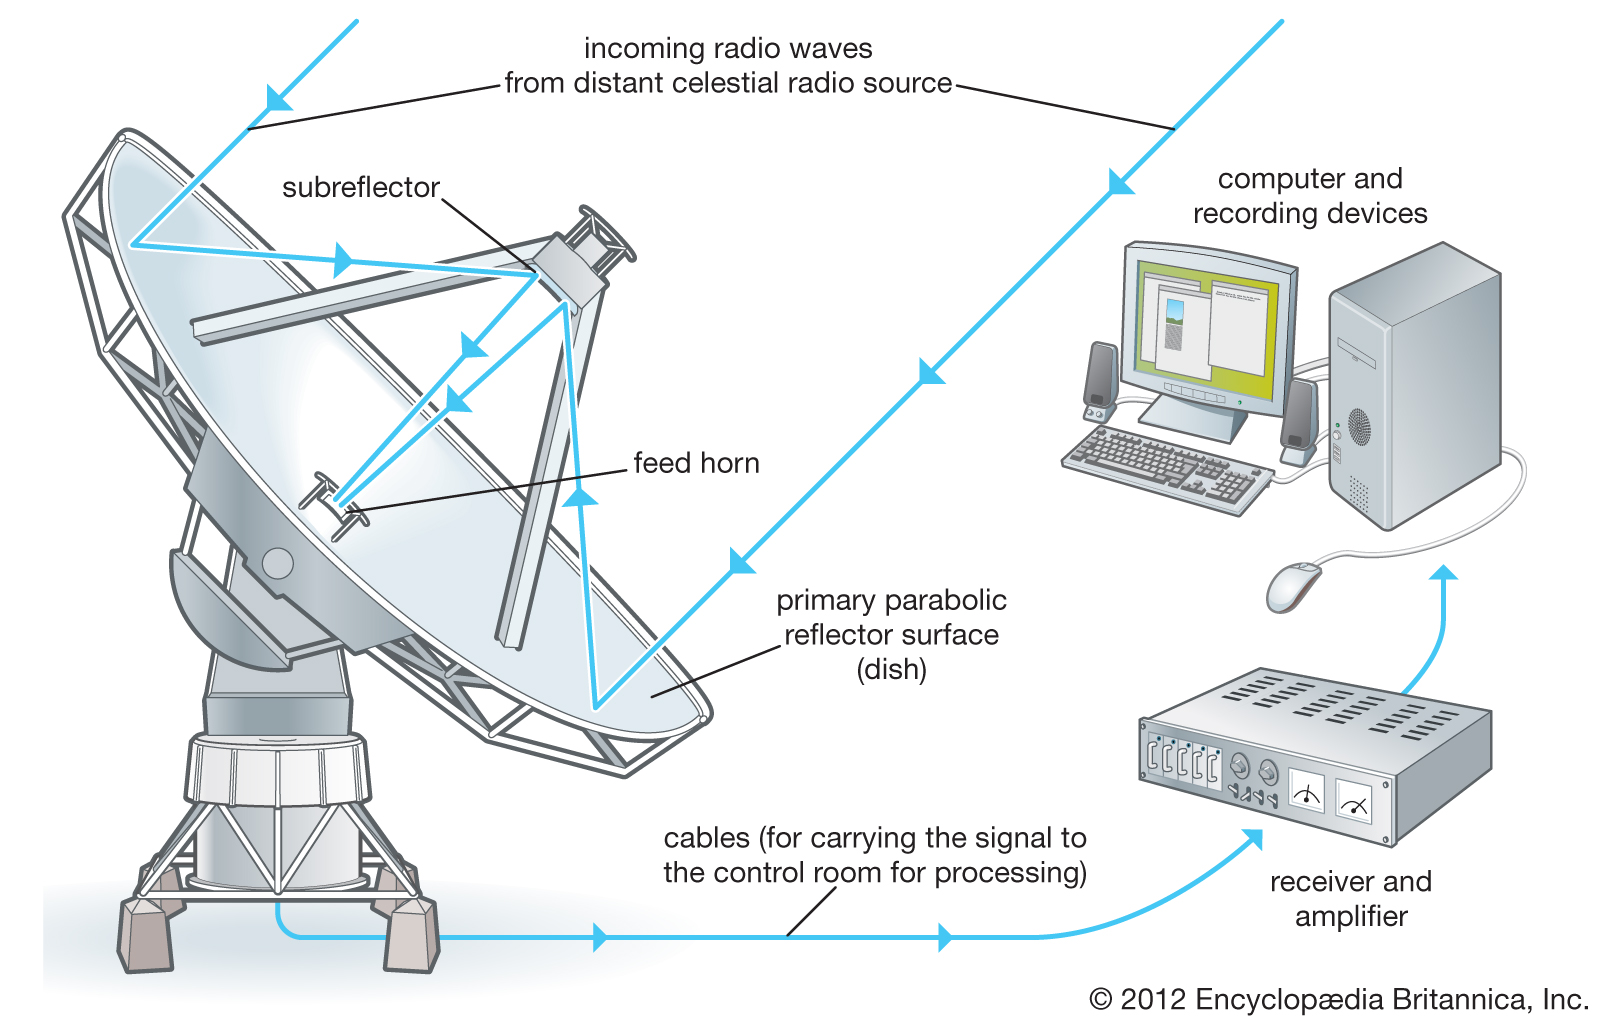
\includegraphics[width=0.5\textwidth]{Images/Telescope.jpg}
	\caption[]{Parabolic reflector antenna design\footnotemark.}
	\label{ra:fig:para}
\end{figure}
\footnotetext{Taken from \url{http://kids.britannica.com/comptons/art-145514}}
%
\subsubsection{Radio Interferometry}\label{ra:ssec:des}
Radio interferometry uses an array of antennas to detect and measure objects emitting radiation in the radio-wave frequencies. Radio waves are defined as electromagnetic radiation with wavelengths of the order of $10^{-3}$ to $10^5$ m \citep{cheng2009radio}. The interferometer finds the source of these waves by detecting correlations in the parallel ray signal transmitted by the radiating source \citep{tasse2016tessellation} and collected by multiple antennas to determine the delay as well as the amplitude and frequency of the source to calculate the position, size and intensity of the source \citep{thompson2008interferometry}.
%
\subsubsection{Radio Telescope Mounts}\label{ra:ssec:mount}
The choice of mount used for a radio telescope plays a large role in how well the telescope is able to track an object. The two main models used are the altazimuth and equatorial mounts. An altazimuth mount rotates on two independent axes, giving it a wide range of motion. The equatorial mount has one axis which is fixed to be parallel to the equator. This allows the antenna to simply move across the sky in one direction to track an object. The equatorial mount also follows the natural rotation of the sky as it passes to obtain less distortion (Section \ref{ra:ssec:eec}) than the altazimuth mount. Altazimuth mounts are still more common as they are relatively cheaper and easier to build than equatorial ones \citep{thompson2008interferometry}.
%
%\subsubsection{The SKA}
%--------------------------------------------------------------------------------------
\subsection{Image Capture and Processing}\label{ra:sec:ic}
%
\subsubsection{Aperture Synthesis}\label{ra:ssec:rii}
The electromagnetic radiation collected by the antenna is correlated into voltage differences. The data are collected and stored over some hours and the resulting correlations in the data taken in by each antenna in the telescope are Fourier transformed from the frequency domain to the spatial domain, to give a two dimensional image \citep{sault1994multi}.
%
\subsubsection{The Primary Beam}\label{ra:ssec:tpb}
The primary beam is a mathematical function that describes the sensitivity pattern of an antenna. Naturally the beam is most sensitive in the center of the direction in which the antenna is facing, with fringes of sensitivity radiating out as shown in Figure \ref{ra:fig:beam}. The circular sensitivity present in Figure \ref{ra:fig:beam} can be seen affecting the uncorrected image present in Figure \ref{ra:fig:uncorr} \citep{thompson2008interferometry}.
%
\begin{figure}[H]
  \begin{subfigure}{0.45\textwidth}
	\centering
	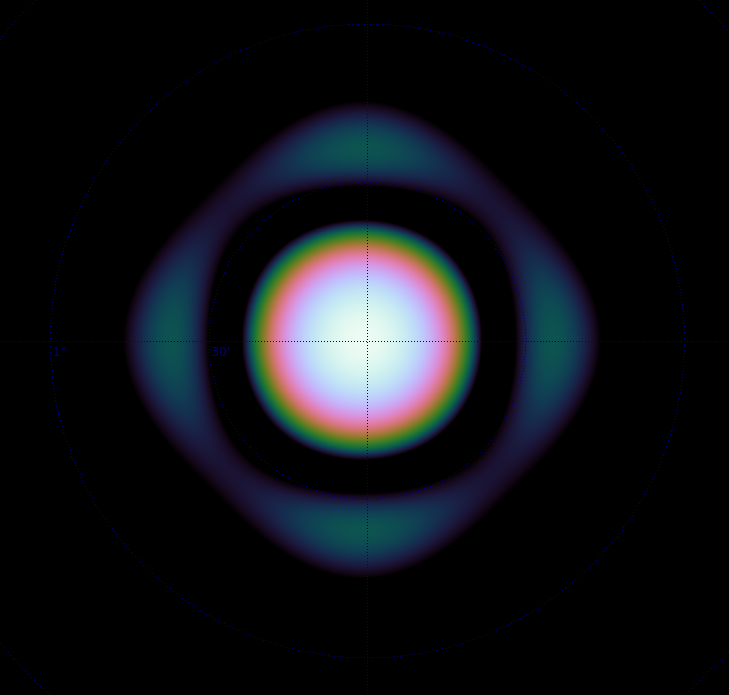
\includegraphics[width=0.9\textwidth]{Images/beam.png}
	\caption{Sensitivity pattern.}
	\label{ra:fig:beam}
  \end{subfigure}
  \begin{subfigure}{0.45\textwidth}
	\centering
	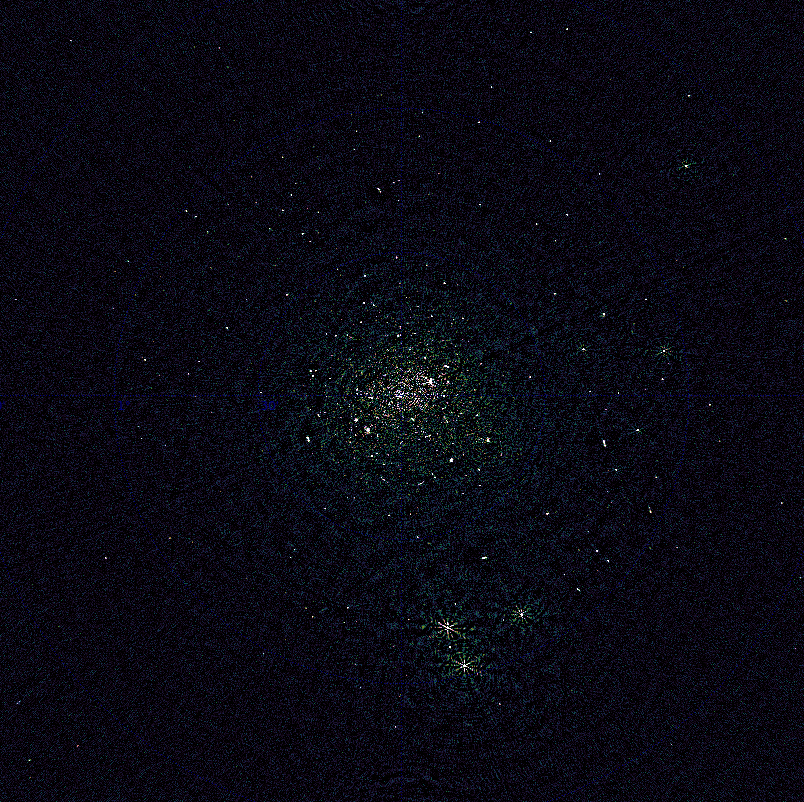
\includegraphics[width=0.9\textwidth]{Images/uncorrected-image.png}
	\caption{Resulting uncorrected image produced through radio interferometry.}
	\label{ra:fig:uncorr}
  \end{subfigure}
  \caption{Primary beam and its effects.}
\end{figure}
%
\subsubsection{Errors and Error Correction}\label{ra:ssec:eec}
As with any real-world data input, the image capturing process of radio interferometry is subject to errors. These errors can be classified as arising from two main groups, namely \gls{di} and \gls{dd} effects \citep{smirnov2011revisiting}. \gls{di} effects are due to differences in the top layer of the atmosphere distorting the signal. This is also known as the complex gain and can be easily corrected for. The \gls{dd} effects in particular arise from distortions due to interference from the ionosphere and deviations of the primary beam from the sky rotation model (due to altazimuth mounts discussed in Section \ref{ra:ssec:mount}). This distortion, $D$, can be corrected, but only relative to a chosen point, $\xi$. The correction at $\xi$ is almost perfect, but as the correction drifts further from $\xi$, it introduces an error which propagates away from $\xi$. This error, $E_i$ at $x_i$ is dependent on the intensity at point $x_i$, $I_i$, and the distortion at the point relative to $\xi$, $D(x_i,\xi)$. Therefore, to minimize this error, every point can be made a correction seed and the image can be broken up according to these points and reassembled to form an image with little to no error. However, this is very computationally intensive as there are thousands of sources per image and the image is sparsely populated. We therefore seek a method that optimises both computational feasibility and error reduction \citep{smirnov2015radio}.
%--------------------------------------------------------------------------------------
\begin{figure}[H]
	\centering
	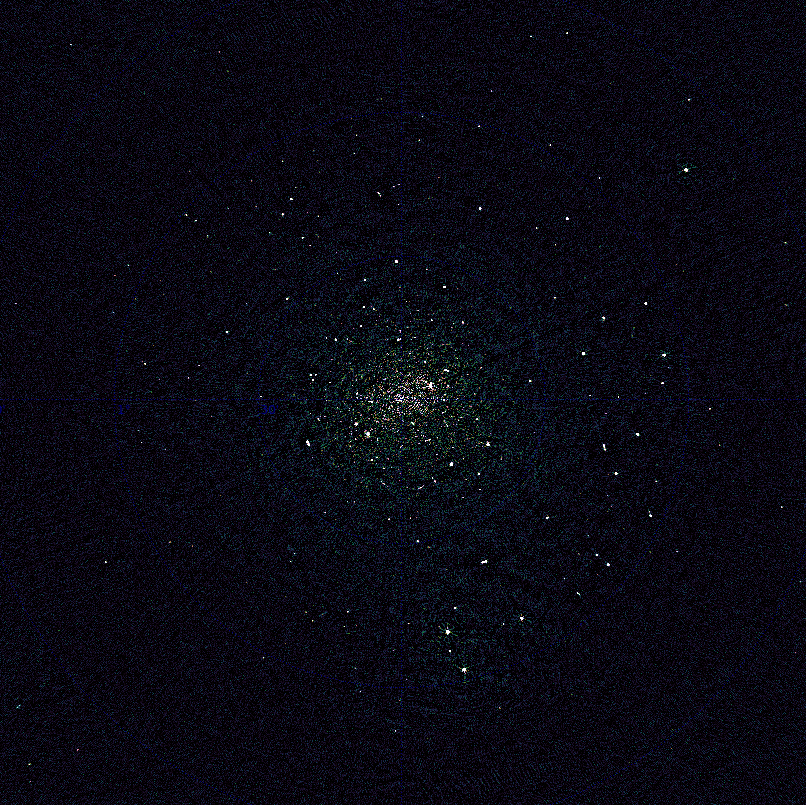
\includegraphics[width=0.5\textwidth]{Images/corrected-23x23.png}
	\caption{Figure \ref{ra:fig:uncorr} corrected on a $23\times23$ grid.}
	\label{ra:fig:cor23}
\end{figure}
\subsection{Naive Method for Error Correction}
The most basic compromise is dividing the image evenly into a grid of smaller images and correcting for these from either the center of the sub-image, the point with the strongest source, or the ``center of mass'' (average location of points) of all the points in the sub-image, either weighted by intensity or not. The problem with this method is that if the sub-image is void and has no definite points or if $\xi$ is set at the center, it could be far from every other point and would have no substantial effect on reducing the overall error. Alternatively, if $\xi$ is set at the strongest source or the center of mass, it could lie too close to the boundary of the sub-image and, again, have no overall impact on error reduction \citep{tasse2016tessellation}. An example of a corrected image can be seen in Figure \ref{ra:fig:cor23}.
%--------------------------------------------------------------------------------------




%\section{Models and Algorithms}\label{tes}
In this section various Voronoi algorithms, namely the incremental, divide and conquer, and Fortune's algorithm are considered, as well as clustering methods for grouping points in a space. Concepts and notation used in the explanation of these algorithms are also discussed
%--------------------------------------------------------------------------------------
\subsection{Voronoi Tessellations}\label{tes:sec:vor}
A Voronoi tessellation is a partitioning of a space $S$ by a set of points. Given $n$ points (seed points) the space, $P = \{p_0,p_2,...,p_{n-1}\}, P \subset S$, is partitioned into $n$ regions, known as Voronoi regions or Voronoi cells, where every point, $s \in S_i,0 \leq i \leq n-1$ in a region, $S_i \subset S$, is closest to a single seed point, $p_i \in P$, in terms of the space's distance measurement operation, $d$ \citep{okabe2009spatial}. An example of a Voronoi diagram is illustrated in Figure \ref{tes:fig:voreg}.
%
\begin{figure}[H]
    \centering
    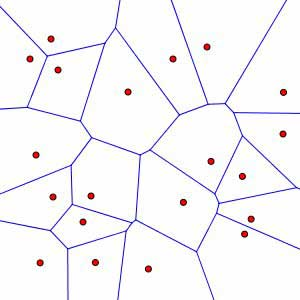
\includegraphics[scale=0.65]{Images/voronoi.jpg}
    \caption[]{Voronoi diagram\footnotemark}
    \label{tes:fig:voreg}
\end{figure}
\footnotetext{Taken from \url{http://www.ams.org/samplings/feature-column/fcarc-voronoi}}
%
\subsubsection{Weighted Voronoi Tessellations}\label{tes:ssec:wei}
The basic form of the Voronoi tessellation has the seed points being indistinguishable from one another, other than having a different position in the space. An extension of the tessellation is with the seeds having some bias or weighting associated with them. These weightings can represent a property of the data, for example, in terms of radio interferometry, they can represent the intensity of each detected source. This weighting can affect $d$ in different ways, depending on how the weighting is accounted for; this is know as the ``weighted distance''. Some of the methods, discussed in \citet{okabe2009spatial} include multiplicative, additive, compound and power Voronoi diagrams. These diagrams have distance operators described below as $d_M$, $d_A$, $d_C$, and $d_P$, respectively.
%
\begin{equation*}
\begin{aligned}
  d_M(s,p_i) &= \frac{1}{w_i}d			\\
  d_A(s,p_i) &= d - w_i				\\
  d_C(s,p_i) &= \frac{1}{w_{i1}}d - w_{i2}	\\
  d_P(s,p_i) &= d^2 - w_i			\\
\end{aligned}
\end{equation*}
%
Problems arise in attempting to compute the tessellations for the multiplicative, additive and compound Voronoi diagrams as the edges of these diagrams could potentially be curved by a circular arc ($d_M$,$d_C$), a hyperbolic arc ($d_A$,$d_C$) or a fourth order polynomial arc ($d_C$) \citep{okabe2009spatial}. This leaves the power diagram as the only Voronoi diagram that enforces straight lines for the edges and the resulting tessellation as a set of convex polygons, similar to the standard Euclidean Voronoi diagram. For the power diagram, if the weighting is equal for all points, the resulting diagram is the same as that of a standard Euclidean Voronoi diagram. It is however possible in the power diagram, that a seed point will not be contained within its own associated Voronoi polygon. This occurs when two seed points ($p_i,p_j \in P$, $w_i<w_j$, $i\neq j$) are close enough together such that the weighted bisector, defined by 
%
\begin{equation}
 b(p_i,p_j) = \frac{1}{2}(||\vec{x}_i||^2-||\vec{x}_j||^2+w_i-w_j) \qquad \vec{x}_i = (x_i,y_i),
\end{equation}
%
does not lie on the line segment $\bar{p_ip_j}$. When this occurs, $p_i$ lies in the region of $V_j$. If the difference in weighting between $p_i$ and $p_j$ is large enough and the distance between them small enough, the points in $V_i$ may be an empty set. It is worth noting that Power Diagrams are also referred to as General Voronoi Diagrams \citep{aurenhammer1987power}.
%--------------------------------------------------------------------------------------
\subsection{Voronoi Tessellation Generation Algorithms}\label{tes:sec:tga}
Although Voronoi tessellations extend to multiple dimensions, for simplicity we only discuss those in a two dimensional plane.
%
\subsubsection{Incremental Algorithm}\label{tes:ssec:inc}
The most simplistic of the generation algorithms, the Incremental is an iterative algorithm as described below \citep{green1978computing} \citep{okabe2009spatial}:
\begin{enumerate}
\item Start from $i=0$ with an empty plane.
\item\label{tes:itm:inc:add} A seed point, $p_i$ is placed into the plane.
\item The nearest neighbouring seed point $p_f=p_{nn}$ is found.
\item\label{tes:itm:inc:bis} A perpendicular bisector is drawn between $p_i$ and $p_f$ (if it exists).
\item The bisecting line is followed in both directions until it intercepts an existing edge or the plane's boundary on both ends.
\item A new edge is defined by this segment of the bisector as part of both $p_i$ and $p_f$.
\item The seed point of the polygon that shares the found edge clockwise to $p_f$ (anticlockwise to $p_i$) is set to $p_f$.
\item Continue from step \ref{tes:itm:inc:bis} until $p_f=p_{nn}$.
\item Set $i = i +1$ and repeat from step \ref{tes:itm:inc:add} until $i=n$.
\end{enumerate}
In its most naive form, this algorithm achieves an efficiency of $O(n^2)$.
%
\subsubsection{Divide and Conquer Algorithm}\label{tes:ssec:dac}
The Divide and Conquer algorithm was first proposed by \citet{shamos1975closest}, but is also described in \citep{okabe2009spatial}. It is a recursive algorithm that improves on the Incremental algorithm by having an execution time of $O(n\log n)$.
\begin{enumerate}
\item If the space contains only one point, return it with the entire plane as its Voronoi region.
\item Divide the space, $S$ containing the set of $n$ seed points, $P$, into two subspaces, $S_L$ and $S_R$, such that $S_L$ and $S_R$ contain $n/2$ seed points and every seed point of $P_L$ lies to the left of every seed point of $P_R$ (this is made easier if $P$ is ordered).
\item Recursively compute the Voronoi tessellations for $P_L$ in $S_L$ and $P_R$ in $S_R$; called $V_L$ and $V_R$, respectively.
\item A polygonal line, $Q$, must now be found such that $Q$ merges $V_L$ and $V_R$ into a single Voronoi tessellation, $V$:
\begin{enumerate}
 \item Start with the polygon of $V_R$ which contains the top-left corner of $S_R$, $p_R$ and the polygon of $V_L$ which contains the top-right corner of $S_L$, $p_L$. Since $p_L$ must lie to the left of $p_R$, they must overlap when $V_L$ and $V_R$ are extended into $S$.
 \item\label{tes:itm:dac:bis} A perpendicular bisector is drawn between $p_L$ and $p_R$ and segmented between its two closest edge intercepts from the shortest distance between $p_L$ and $p_R$. This segment is added to $Q$.
 \item If the lower edge, intercepted by the bisector is in $V_R$, $p_R$ is set to the seed point polygon which shares this edge and similarly if the edge is in $V_L$.
 \item Continue from step \ref{tes:itm:dac:bis} until the bottom of $S$ is reached.
\end{enumerate}
\item Remove all line segments of $V_L$ to the right of $Q$ and all those of $V_R$ to the left of $Q$ to form $V$.
\item Return $V$ recursively until the full Voronoi tessellation is complete.
\end{enumerate}
Part of achieving this efficiency is assuming $P$ is co-lexicographically ordered, meaning for all $p_i,p_j \in P$, $0 \leq i < j < n$; $x_i > x_j$ or $(x_i = x_j$ and $y_i > y_j)$. This speeds up the partitioning of $P$ into $P_R$ and $P_L$ at each level of recursion.
%
\subsubsection{Fortune's Algorithm (Sweep-Line Method)}\label{tes:ssec:fort}
\citet{fortune1987sweepline} describes an algorithm where the tessellations are found by a line ``sweeping'' over the space and solving the problem at each step of the sweep. This can be problematic for Voronoi tessellations as the line may intercept the Voronoi region of a seed point before it intercepts the point. Therefore the Voronoi tessellation is not computed directly, but through a geometric transform. The transform $\phi(x(s),y(s))$ works such that for any point, $s \in S$ with coordinates $(x(s),y(s))$, 
\begin{equation}
  \phi(x(s),y(s)) = (x(s) + r(s), y(s)),
\end{equation}
where $r_i(s)$ is defined as the distance to the seed point $p_i \in P$ and $r(s) = min\{r_i(s) | 1 \leq i \leq n-1\}$, is the distance to the closest seed point to $s$. This transform can easily be reversed to re-obtain $S$ and its set of Voronoi tessellations. Now, for the transform of $S$, $\phi(S)$ denoted by $\Phi$, the left-most point of each Voronoi Region is its seed point (except the left-most seed point); this is essential for the algorithm. It is important to note that the perpendicular bisectors of seed points in $S$, through the transform, become hyperbolas in $\Phi$ (provided they are not horizontal in $S$). For $p_i,p_j\in P$, the hyperbola is denoted as $h_{ij}$ which can be split into $h^+_{ij}$ and $h^-_{ij}$ as the upper and lower half-hyperbolas about the left-most point, respectively. Set $Q$ is denoted as the set of all event points in the algorithm. $Q$ is initially populated with the seed points (in co-lexicographical order) but the edge interceptions are added as they are found. The algorithm, as described by \citet{okabe2009spatial} is as follows:
\begin{enumerate}
  \item Add $P$ to $Q$.
  \item Choose and delete the leftmost seed point, $p_i$ from $Q$.
  \item Create a list, $L$ containing the transformed Voronoi region of $p_i$, $\phi(V_i)$.
  \item\label{tes:itm:for:q} While $Q$ is not empty do the following:
  \begin{enumerate}
    \item Choose and delete the leftmost element, $w$ of $Q$.
    \item If $w$ is a seed point:
    \begin{enumerate}
      \item Set $p_i=w$.
      \item Find the region, $\phi(V_j)$, containing $p_i$.
      \item Replace $\phi(V_j)$ in $L$ with $(\phi(V_j),h^-_{ij},\phi(V_i),h^+_{ij},\phi(V_j))$.
      \item Find the half-hyperbola intercept(s) with any other hyperbolas, if they exist, and append these to the front of $Q$.
      \item Repeat from step \ref{tes:itm:for:q}.
    \end{enumerate}
    \item If $w$ is a half-edge:
    \begin{enumerate}
      \item Set $\phi(q_t)=w$ where $\phi(q_t)$ is the intercept of $h^\pm_{ij}$ and $h^\pm_{jk}$.
      \item Replace all sequences of the form ($h^\pm_{ij},\phi{V_j},h^\pm_{jk}$) on $L$ with $h=h^+_{ik}$ or $h=h^-_{ik}$ appropriately.
      \item Remove from $Q$ any intersections of $h^\pm_{ij}$ and $h^\pm_{jk}$ with other half-hyperbolas.
      \item Move any intersections of $h$ in $L$ to $Q$.
      \item\label{tes:itm:for:mark} Mark $\phi(q_t)$ as a Voronoi vertex incident to $h^\pm_{ij}$, $h^\pm_{jk}$ and $h$.
      \item Repeat from step \ref{tes:itm:for:q}.
    \end{enumerate}
  \end{enumerate}
  \item Return the half-hyperbolas on $L$, the set of marked intersections from step \ref{tes:itm:for:mark} and the relations among them.
\end{enumerate}
%--------------------------------------------------------------------------------------
\subsection{Clustering Algorithms} \label{tes:sec:clu}
It may be the case that the number of potential seed points in a space, $N_p$, is much larger than the optimal number of facets, $N_v$. In these cases the overall computation time would be drastically reduced if the $N_p$ points were grouped into $N_v$ clusters. From each of these clusters, a point is chosen as a seed point to be used to find the corresponding Voronoi tessellation. Some key examples of such clustering algorithms are described in this subsection.
%
\subsubsection{K-Means Algorithm}\label{tes:ssec:kma}
K-means clustering is an iterative process where an initial guess at the center of a cluster, $c$, is made and improved with each iteration. It is named as such because it seeks to separate $n$ objects into $k$ clusters where, for each object in a cluster $( o^i \in C_i$, $i \in \mathbb{R}$, $0\leq i \leq k-1)$ the mean point of that cluster, $c_i$, is closer to it than any other mean point and the $c_i$ is representative of the average values of all points, $\frac{1}{m}\sum^m_{j=1}o^i_j$, in $C_i$. \citet{way2012advances} describe the algorithm as follows:
\begin{enumerate}
  \item	Randomly choose $k$ mean points $(c_0,\dots,c_{k-1})$.
  \item\label{tes:itm:km} Assign each $c_i$ an empty object set, $C_i$.
  \item Iterate through all the objects in the space $(o_0,\dots,o_{n-1})$ and assign the object to the object set of the mean point closest to it.
  \item Set all $c_i$ to be the average of all points in their respective $C_i$.
  \item If the sum of the changes in $c_i$, $\sum_0^{k-1} \Delta c_i$, is greater than some given tolerance, $\epsilon$, the algorithm is repeated from step \ref{tes:itm:km}, else return the set of means (and their object sets if 	      necessary).
\end{enumerate}
One obvious problem with this algorithm is that the number of iterations can be unpredictable; this is addressed by having the sum of changes only converge to $\epsilon$, instead of complete convergence. With large data sets and large $k$-values where the mean points converge in smaller steps with every iteration, this can drastically reduce the runtime of the algorithm. The clusters produced are also dependent on the initial placement of the mean points \citep{way2012advances}. Other methods of improving the runtime include probabilistic choices of starting mean points \citep{arthur2007k} and constraining the distance and using the triangle inequality \citep{hamerly2010making}.
%
\subsubsection{Bisecting K-Means Algorithm}\label{tes:ssec:bkma}
A variation on the k-means algorithm is to embed it into another iterative method, which, by design, reduces the computation time and also improves the quality of the clusters produced. The algorithm works by branching large clusters into smaller ones. The algorithm, described by \citet{steinbach2000comparison}, is as follows:
\begin{enumerate}
  \item Start with the entire set of objects in the space as part of a single cluster.
  \item\label{tes:itm:bkm} Choose the largest cluster in the space.
  \item Split the objects into two sub-clusters and refine iteratively by way of the k-means algorithm.
  \item Repeat from step \ref{tes:itm:bkm} until $k$ clusters are produced.
\end{enumerate}
%
\subsubsection{Agglomerative Clustering Algorithm}
Differing from the k-means algorithm (and more specifically the bisecting k-means) is the agglomerative clustering algorithm. Instead of starting with a single cluster containing all points, this algorithm instead places every point in its own cluster and merges them until the required number of clusters are produced. \citet{way2012advances} describe the algorithm as:
\begin{enumerate}
  \item Begin with each object in its own cluster.
  \item\label{tes:itm:aca} Merge the two closest clusters.
  \item Repeat step \ref{tes:itm:aca} until $k$ clusters remain.
\end{enumerate}
Although this algorithm will always yield the same result for a given data set, it is far more expensive than the k-means. Improvements can be made on this, however by instead building a minimum spanning tree, weighted by the distance between the data and iteratively removing the links with the highest weights until the number of required clusters is produced.
%--------------------------------------------------------------------------------------
\subsection{Related Work}\label{ra:sec:rw}
%
\subsubsection{Standard Voronoi Faceting}\label{ra:ssec:svf}
In \citep{tasse2014applying}, \citep{smirnov2015radio} and \citep{van2016lofar}, a series of observed or simulated extragalactic points are clustered into facets using a Voronoi tessellation algorithm with the seed points for these facets set as the brightest points in each facet. An example of this can be seen in Figure \ref{tes:fig:stelvor} where the facets are superimposed over the source image from which they are derived.
%
\begin{figure}[H]
    \centering
    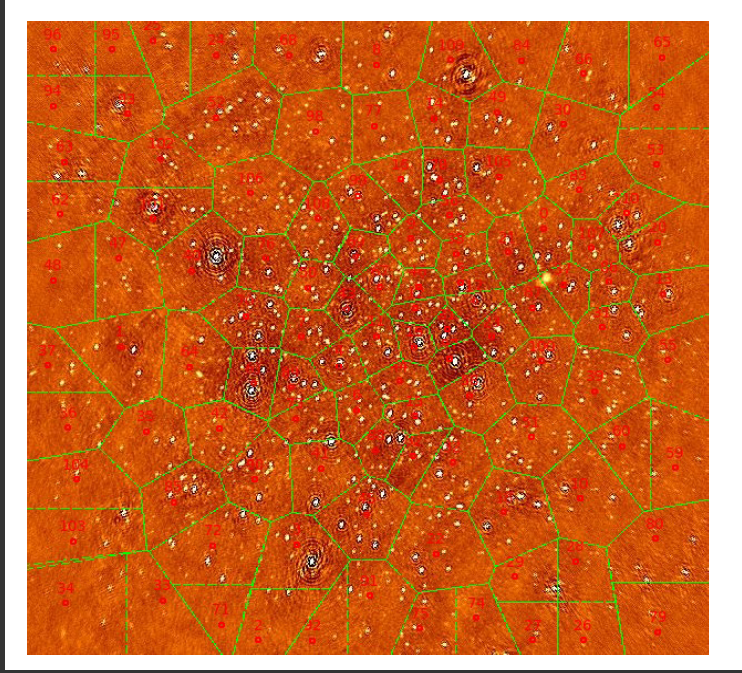
\includegraphics[scale=0.4]{Images/tessellation.png}
    \caption{Example of Voronoi faceting to group extragalactic points for Direction Dependant calibration.}
    \label{tes:fig:stelvor}
\end{figure}
%--------------------------------------------------------------------------------------
%\section{GPU Architecture and Concepts}\label{gpu}
In this section the history of GPUs from their initial use for pixel generation in gaming to the parallel data processing titans they are today is looked at. More specifically we focus on the NVIDIA GTX 750 Ti, and how its GM107 architecture has improved to give high performance with low power consumption. The GPU programming language, CUDA, is discussed as well as CUDA best practices for optimizing the run time of the code.
%--------------------------------------------------------------------------------------
\subsection{Parallelism}\label{gpu:sec:par}
One of the main means of reducing processing time is through parallelism. The two main forms of parallelism are task and data parallelism. Task parallelism can be seen as running multiple processes concurrently where communication between the processes is explicitly defined to avoid race conditions \citep{subhlok1993exploiting}. Data parallelism is the distribution of a data set over a number of identical processes each of which performs operations on a unique subset of the data. Race conditions occur when parallel processing streams access data or perform operations out of the intended order, leading to errors or incorrect output being produced. A combination of task and data parallelism can lead to an ideal speed-up, but both have their limits depending on the task and the data being operated on \citep{subhlok1993exploiting}.
\\
\\
The increased need for parallelism came about in 2005, when \gls{cpu} frequency peaked at 4 GHz due to heat dissipation issues. However, Moore's Law \citep{moore2006cramming}, still holds, and is still expected to hold until 2025 (that is, that the number of transistors in a processor will double every two years). This leads to a problem where the speed at which an operation is done cannot be increased (due to the frequency limit), but the number of concurrent operations can still increase. This means that the only way to speed up an operation is to change it from a sequential to a parallel process \citep{rajan2013informatics}.
%--------------------------------------------------------------------------------------
\subsection{GPU Execution}\label{gpu:sec:opt}
\gls{gpu}s were originally designed for rendering pixels and vectors in games. They were especially designed for this since \gls{cpu}s are optimized to run sequential instructions as fast as possible, whereas pixel and vector calculations are inherently parallel. With NVIDIA's release of CUDA in 2006, \gls{gpgpu} programming became feasible as a way to accelerate data processing using both data and task parallelism through the simultaneous execution of similar tasks \citep{cuda_home}.
\\
\\
The power of a \gls{gpu} stems from its architecture which is optimized for a special case of \gls{simd} processing known as \gls{simt}. \gls{simd} allows a central processor to distribute a set of instructions to multiple simple processors which act on the data simultaneously. \gls{simt} is more generalized as each warp (Section \ref{gpu:ssec:smm}) of the \gls{gpu} can perform different tasks given the same set of instructions. This is due to the way in which the \gls{gpu} handles branching at the thread level. By exploiting these processes, and this instructional architecture, some instructions can be computed faster than is possible on a  a \gls{cpu} \citep{vuduc2013brief}.
%--------------------------------------------------------------------------------------
\subsection{The NVIDIA GeForce GTX 750 Ti}\label{gpu:sec:750}
%
\subsubsection{GM107 Maxwell Architecture}\label{gpu:ssec:max}
The NVIDIA GeForce GTX 750 Ti \gls{gpu} was released on the 18th of February 2014. It boasts 640 CUDA cores, 1020 MHz base clock speed, 1305.6 GFLOPs and a memory bandwidth of 86.4 GB/sec. It is NVIDIA's first-generation Maxwell architecture, designed for high performance at relatively low power consumption (60 W) and has the codename 'GM107'. The \gls{gpu} uses PCI Express 3.0 to interface with the host machine through the GigaThread engine. The first-generation Maxwell (from now simply referred to as Maxwell) is made up of one \gls{gpc} on which the processing occurs. It also contains a large L2 cache at 2048 KB and two 64-bit memory controllers to access the 2048 MB global memory. This design can be seen in Figure \ref{gpu:img:gm107} \citep{geforce_750}, \citep{g750_paper}.
%
\begin{figure}[H]
 \centering
 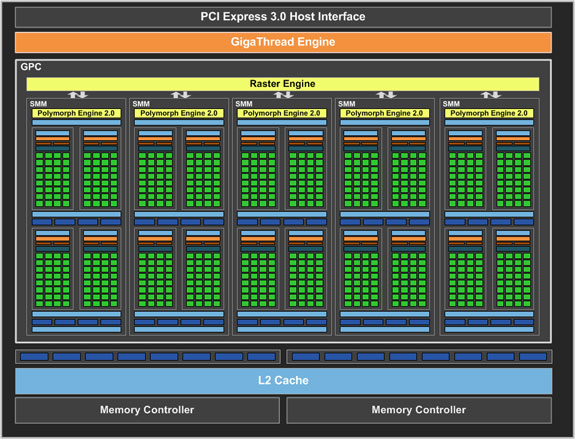
\includegraphics[width=0.5\textwidth]{Images/GM107.jpg}
 \caption[]{NVIDIA Maxwell Architecture.\footnotemark}
 \label{gpu:img:gm107}
\end{figure}
\footnotetext{Taken from \url{http://www.hitechlegion.com/reviews/graphics}}
%
\subsubsection{Streaming Multiprocessors}\label{gpu:ssec:smm}
The \gls{gpc} is further broken down into five \gls{sm}s which are divided into four processing blocks. The processing blocks (or warps) each contain an instruction buffer, a scheduler and 32 CUDA cores as seen in Figure \ref{gpu:img:smm}. These warps are set in a lock step, meaning each core in a warp executes the same set of commands at the same time, with different valued variables \citep{CUDA}.
%
\begin{figure}[H]
\centering
 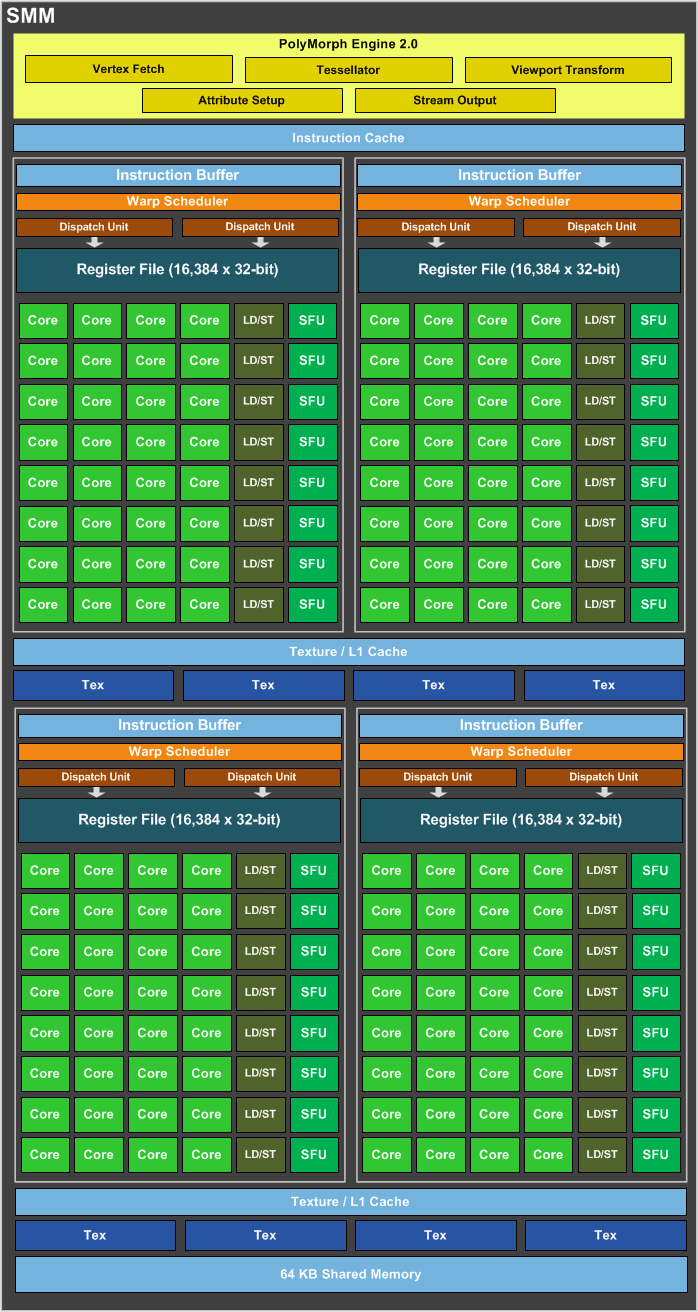
\includegraphics[width=0.3\textwidth]{Images/GM107SMM.png}
 \caption[]{Maxwell Streaming Multiprocessor.\footnotemark}
 \label{gpu:img:smm}
\end{figure}
\footnotetext{Taken from \url{http://www.legitreviews.com}}
%--------------------------------------------------------------------------------------
\subsection{CUDA}\label{gpu:sec:cuda}
CUDA is a parallel programming language created by NVIDIA for the purpose of running on their brand of \gls{gpu}s. CUDA was modelled as a C-like language with some C++ features. Its main feature is the way in which it separates \gls{cpu} and \gls{gpu} code. The \gls{cpu} code is labelled as ``host'' code and the GPU's as ``device'' code. Device code is called by the host through a special case of a method, known as a kernel. The basic structure of a kernel is as follows: 
\\
\\
\texttt{kernel0<<<grid, block>>>(params);}
\\
\\
In this instance \texttt{kernel0} would be the name of the kernel being called, \texttt{grid} is the three dimensional value of the number of blocks to be assigned, \texttt{block} being similar to \texttt{grid} is a three dimensional value of the number of threads needed and \texttt{params} is simply the parameters needed by the kernel to execute (similar to those of a method) \citep{CUDA}.
%
\subsubsection{Threads}\label{gpu:ssec:thread}
The thread is the smallest processing unit of the \gls{gpu}. \gls{gpu} threads are designed to be cheap and lightweight compared to those of a \gls{cpu} so that a thread can easily be created, run its small task and be destroyed to make place for the next thread. Threads are arranged into \gls{3d} blocks with each thread having a unique \gls{3d} ID within that block, namely an x, y and z ID. Generally the thread ID is used as the means of determining the difference in the task process of each thread \citep{CUDA}.
%
\subsubsection{Blocks}\label{gpu:ssec:block}
Each block may have a maximum of 2056 threads in total and 1024 for any single dimension; this is the reason why they are bundled into a larger, \gls{3d} grid structure. Similarly to threads, blocks have a unique \gls{3d} ID in the grid. While warps execute each step of a process simultaneously, this is not necessarily true for blocks when spread over multiple warps. More often than not, blocks exchange data within their threads and if precautions such as thread synchronisation are not taken, race conditions could ensue to break the code. Each block, when executing, must occupy a whole number of warps (rounded up). This is done as warps are constantly in lock step. Threads within a block share a fast memory, located in the L1 cache of the streaming multiprocessor. This shared memory must be preallocated when the kernel is called as a third parameter within the kernel launch (parameters within the triple angle brackets) \citep{CUDA}.
%
\subsubsection{GPU Memory Hierarchy}\label{gpu:ssec:mem}
In order to maximize concurrency on the card, the \gls{gpu} has a structured memory hierarchy. The largest, slowest and most generally accessible of these is the global memory which resides on the device memory. This memory is visible to every thread and also to every kernel called in one application. 
\\
\\
The constant memory also resides on the device memory; as the name suggests, values stored here cannot be altered and are read-only until the space is deallocated. Variables stored in constant memory also have the ability to broadcast their values to multiple threads simultaneously.
\\
\\
Similar to constant memory, texture memory also lies on the device memory and is also read-only; it is optimized for storing 2D arrays where multiple neighboring values of the array can be read concurrently.
\\
\\
The shared memory lies on the SM and is visible only to a block as a means for threads within a block to exchange data. Shared memory must be declared with the size of the memory needed (up to the maximum $64$ Kb) when the kernel is executed.
\\
\\
Each processor is assigned its own memory space to be used by each thread, in the form of registers. Registers are visible only by the thread currently on that processor and reset with each change of thread. Registers hold the variables created in and passed to the thread. The register is by far the smallest memory on the card at 32 bits per register, but 255 registers per thread. Should the thread call too many variables or variables too large to fit in the registers, the variables spill over into local memory, which lies in the L1 and L2 caches for active threads. Should the thread need to be temporarily halted for another thread to use the processor, the thread's variables are stored in local memory on the device memory \citep{CUDA}. A visual description of the memory hierarchy can be seen in Figure \ref{gpu:img:mem}.
%
\begin{figure}[H]
\centering
 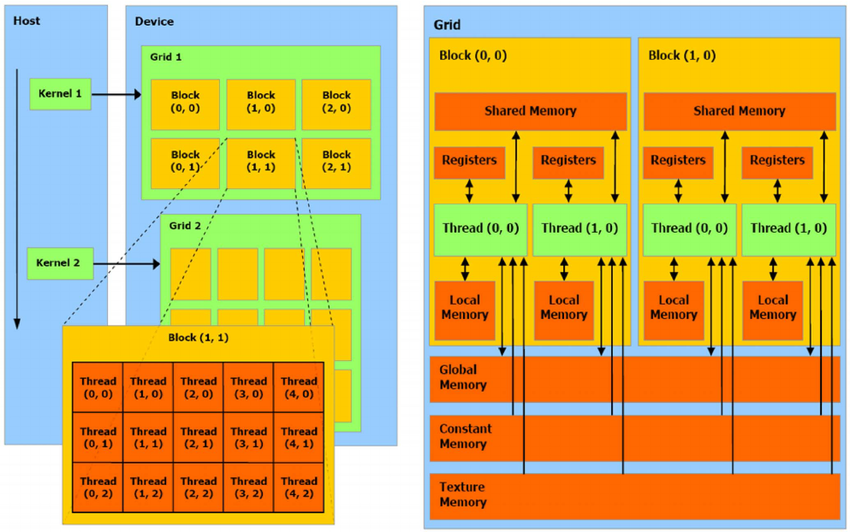
\includegraphics[width=0.7\textwidth]{Images/Cuda_mem_struct.png}
 \caption[]{CUDA memory hierarchy.\footnotemark}
 \label{gpu:img:mem}
\end{figure}
\footnotetext{Taken from \url{https://www.researchgate.net}}
%
\subsection{CUDA Optimization}\label{gpu:sec:cop}
As stated in Section \ref{gpu:sec:opt}, GPUs are designed for parallel computing to speed up the execution of a process when compared with running it on a CPU. To ensure the greatest speed-up a variety of optimizations are typically necessary to improve naive parallel code. These optimizations can be categorized into three groups, memory, execution configuration and instruction optimizations. The NVIDIA Visual Profiler (NVVP) is invaluable in assisting users to identify areas in their CUDA code that require optimization.
\subsubsection{Memory Optimization}
Memory optimization seeks to maximize the bandwidth of the GPU so that more time is spent using the faster memory (e.g. registers, L1 and L2 caches) and less time on the slower memory (e.g. device memory, host memory). An example of a memory optimization is that CUDA has the ability to asynchronously transfer data between the host and device by breaking a kernel into streams, thereby allowing the device to process one section of the data while another is still being transferred to it and a third is being transferred back to the host. Alternately, memory on the host can simply be mapped to the device. This memory is accessible by both the host and device and is known as zero-copy memory. This can only be done on pinned memory, which is memory set aside by CUDA to be used by the GPU, and is also optimized to have a higher transfer rate to the GPU than any other host memory. This can be taken a step further through unified virtual addressing, where the host and device share a single virtual memory space; this address space lies on the host, but through predictions by CUDA on the need for certain sections of the memory, parts of the memory are transferred to the device as they are needed. The different types of memory found in the GPU as discussed in Section \ref{gpu:ssec:mem} show examples of this as well. Constant and texture memory, for example, improve latency by having the value broadcast to all threads and 2D spatial locality read abilities, respectively. The use of sequential reads and stride accessing can also improve bandwidth usage as the memory required is aligned on the device \citep{CUDA}.
%
\subsubsection{Execution Configuration Optimization}
Execution configuration optimizations seek to improve the overall usage of cores on the GPU, keeping as much of the hardware as possible occupied to improve the overall execution time. One way of achieving this is through concurrent kernel execution, that is, multiple kernels running concurrently to reduce the idle time of each warp. Another way is by setting the number of threads in a block to always be a multiple of 32 so that all the cores in a warp are occupied. Other examples include having multiple small blocks instead of a single large block, especially when using thread synchronizations and also having a minimum block size of 32 threads \citep{CUDA}.
%
\subsubsection{Instruction Optimization}
Instruction optimization uses the knowledge of how certain instructions are executed to speed up code in critical areas. This form of optimization is most prevalent in arithmetic operations. Most notably, single precision is encouraged as well as using the multiple CUDA maths libraries that interface directly with the hardware. These libraries include cuBLAS for linear algebra, cuSparse for sparse matrix operations, cuRAND for random number generation, nvGRAPH for graph analytics and cuFFT for fast Fourier transforms. These and more libraries are discussed in \citep{CUDA_lib}. Another way of reducing latency is by minimizing the use of global memory, as it is generally the slowest to access. Making use of constant and shared memory for read-only values and shared memory for block specific values can drastically improve memory access times \citep{CUDA}.
%--------------------------------------------------------------------------------------
\subsection{Related Work}\label{gpu:sec:rel}
Only one study relating to GPU implementation of a Voronoi tessellation has, to the best of our knowledge, been published. This algorithm is called "Jump Flooding" and is explained below.
\\
\\
\citet{rong2006jump} describe a method of approximating a Voronoi transform using a method known as jump flooding. The algorithm works by seeing the space as a discrete $n \times n$ grid. It works by having grid cells with an identified closest seed point (or in this case, seed cell) and projecting this seed cell to surrounding cells without an identified seed cell in incrementally smaller steps, starting from a step size of $n/2$.
\\
\\
While the Jump Flood does outperform standard CPU algorithms, it is sensitive to the resolution of the output grid. Therefore the algorithm could potentially be slower than a CPU implementation where the CPU implementation is grid independent, such as the divide and conquer or Fortune's algorithm.
%--------------------------------------------------------------------------------------
%\section{Summary}\label{sum}
In this chapter we have discussed many of the technical and theoretical aspects used in this study. We began by looking at radio astronomy and how radio telescopes are designed as parabolic arcs. We reviewed Voronoi diagrams and discussed how power diagrams are the natural extension thereof when weights are incorporated. We looked at three clustering algorithms, namely the k-means, the agglomerative, and the bisecting k-means algorithms. Lastly we looked at GPUs, their architecture, and some of the concepts involved. We discussed parallelism and how it has become a necessity due to the physical limitations of individual processors.
\\
\\
At each stage we also looked at existing models, similar to what has been proposed. We looked at the naive grid method for DD-effect error correction and its shortcomings due to empty blocks and off-center optimal points. We discussed a standard Voronoi model for use in the correction of DD effects, saw how it improved on the naive method, but also how it fell short by only regarding the brightest points which may lie too close to one another and warp the entire polygon. Finally, we looked at the jump flood algorithm as a GPU based Voronoi tessellation algorithm. This algorithm approximates a tessellation by changing the space to a grid of finite cells and uses decremental steps to generate a tessellation in a reasonable time.
%--------------------------------------------------------------------------------------

%Include Chapter 3
\chapter{WIP}
\section{Source Selection}\label{sec:design:source}
We begin the algorithm with a list of $n$ sources in the plane. Each source has three parameters: $x$, $y$ and $z$. The $x$ and $y$ parameters define the spatial coordinates of the source while the z parameter is used to reflect the intensity of the source.
\\
\\
The sources are read in and are used to generate the Voronoi centres. Each centre has the following attributes:
\begin{enumerate}
\item An $x$, $y$, and $z$ value inherited from its source.
\item A Boolean value to determine if it is the circumcentre which defaults to false.
\item A centre clockwise to it if it lies on the convex hull which defaults to none.
\item A centre counter-clockwise to it if it lies on the convex hull which defaults to none.
\item A list of all its neighbouring points and the line that bisects them set into a tuple; the list is set to none by default.
\item A list of sources in the cell created by the centre which is set to none by default.
\item The cell's error which is set to zero by default as there are no sources at initialisation.
\item A list of all the cells that have been merged with this cell; by default, this is also set to none.
\end{enumerate} 
Sources are chosen as centres for a Voronoi cell if they have an intensity greater than some predetermined threshold. Once the set of centres, $C= \{c_0,c_1,...,c_n\}$, is created, it is sorted in lexical order i.e. by the $x$ values followed by the $y$ values if the $x$ values are equal. Once the centres have been created, generation of the Voronoi tessellation can begin.
\\
\\
For the sake of testing the system, the $x$ and $y$ coordinates of the sources were randomly generated on a $600 \times 600$ plane with the intensities, $z$, randomly generated as the absolute value of a random normal distribution, centred at zero with a standard deviation of $3000$. Using this, $10000$ sources were randomly generated. From these sources, we generated the centres to be used by the Voronoi, where these centres were sources with an intensity greater than one standard deviation of the mean. Since the absolute value of the source intensity was used, this includes all sources with an intensity greater than 3000, thus accounting for approximately $32\%$ of the sources.
\begin{figure}[H]
\centering
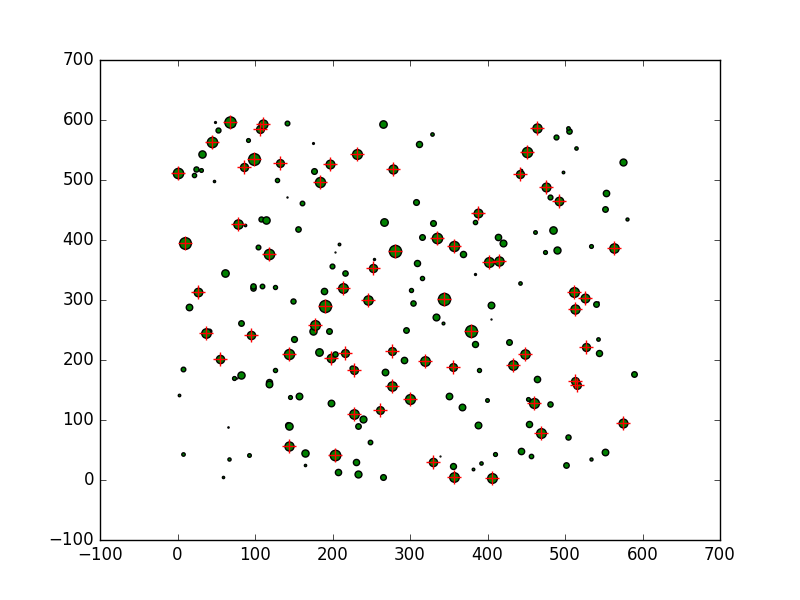
\includegraphics[width=0.8\textwidth]{Images/sources.png}
\caption{ All sources (green circles) with those selected as centres (red crosses).}
\label{fig:source}
\end{figure}
Figure \ref{fig:source} shows sources in green with their intensities represented by the size of the circle on the plane; for simplicity, only $200$ points were generated. The crosses in red represent the centres that were used to generate the Voronoi tessellation.

\section{Voronoi Tessellation Generation}\label{des:sec:vor}
The current best model for creating a Voronoi tessellation uses k-means clustering on all the points in a discrete space to the centres. For every point (the plane is seen as a finite number of pixels) in the plane, $p$, it finds the centre, $c_i$, which is the shortest distance from it, i.e. such that $\sqrt{\big(p(x)-c_i(x)\big)^2 + \big(p(y)-c_i(y)\big)^2}$ is minimised. This is suboptimal as the time taken to create the tessellation relies on the dimensions of the plane and the number of centres therein. Instead we seek a method which is invariant of the plane size and relies solely on the centres. For the sake of decreasing the computation time, this method must also be parallelisable. 
\\
\\
To satisfy these constraints, the divide and conquer algorithm (Section \ref{tes:ssec:dac}) was chosen. The algorithm works by ordering the centres lexicographically and dividing the centres into two subsets, left, $C_L$, and right, $C_R$. The Voronoi tessellations are generated for the left and right subsets separately using the divide and conquer method. The convex hulls of the left and right Voronoi tessellations are then found. The lowest common support line between the hulls is calculated and from this a dividing polygonal chain is generated until it intercepts the upper bounds of the plane. The intersecting edges with the polygonal chain are determined, and lines in the polygonal chain are cut to become part of the Voronoi cells edges.
\\
\\
Code for the Divide and Conquer algorithm was adapted from that in the git repository pyVoronoi\footnote{https://github.com/twmht/pyVoronoi}. pyVoronoi is an implementation for the Divide and Conquer Voronoi algorithm written in Python 2.7. It uses a simple GUI to generate a Voronoi tessellation in a fixed plane using sources read in from a text file. This interface, while simple to use, is constraining as it does not allow users to specify their own spacial constraints or generate the Voronoi as part of a pipelined process. The visualiser and interface were therefore removed and the remaining code re-factored so that the process is a function that can be called by the user or used in a larger process.

\subsection{Structures Used by the Voronoi}\label{sec:des:struct}
The Voronoi structure consists of two main structures, lines and centres. Centres (Section \ref{sec:design:source}) are mainly used to define the sources, but are also used to generate lines.
\\
\\
A line is made up of the following attributes:
\begin{enumerate}
\item Two points, defined as centres which make up the end points of the line. These are defined when the line is created.
\item Two centres which the line bisects, which is set to be empty by default.
\item A centre defining the circumcentre of the line which is empty when the line is created.
\item A list of all lines connected to this one which is used during the merge of the divide and conquer and is empty by default.
\item A Boolean value determining whether the line is active or deprecated. This is set to true by default, but is updated when two cells are no longer neighbours, generally as a result of a merge.
\end{enumerate}

\subsection{Voronoi Function}
The Voronoi function takes in the set of centres and a range of centres it will operate on (initially the entire set, $C$). Depending on the number of points in the subset range, one of three operations occurs.
\\
\\
If the range is made up of more than three points, the range is divided into two equal subranges: one from the starting point of the range to the median, $C_L = \{0,...,\frac{n}{2}\}$ where $n$ is the range, and another from the point after the median to the end of the range,$C_R = \{\frac{n}{2}+1,...,n\}$. The Voronoi function is called again for each subrange, denoted as $C_L$ and $C_R$ for left and right subranges respectively, with the full set of points. Once the Voronoi structures for these two have been calculated, the merge function is called with $V_L$ and $V_R$, the Voronoi structures of $C_l$ and $C_R$ respectively, and the function ends as it is not value returning.
\\
\\
If the range is three, the function generates three bisecting lines, $b_{1,2}$, $b_{1,3}$ and $b_{2,3}$ one for each pair of the three points, $c_1$, $c_2$ and $c_3$. The intercept of $b_{1,2}$ and $b_{1,3}$ is determined. If it does not exist, the centres are collinear and an invalid line exists, and the line, $l_{1,3}$ is removed as, lexicographically, $c_2$ must lie between $c_1$ and $c_3$ and $l_{1,3}$ must therefore lie in the cell of $c_2$. If the intercept does exist, it lies on the circumcentre, $cc$, of the triangle formed by the centres and the lines $l_{1,2}$, $l_{1,3}$ and $l_{2,3}$ with the centres as endpoints. The lines, $l_{1,2}$, $l_{1,3}$ and $l_{2,3}$, are ordered by the square of their lengths and the triangle they form is determined as either acute, obtuse or right-angled. The centres and corresponding lines are appended to each centre's list of related centres, e.g. $(c_2,b_{1,2})$ and $(c_3,b_{1,3})$ are appended to $c_1$'s list of related centres. The bisecting lines, $b_{1,2}$, $b_{1,3}$ and $b_{2,3}$, are clipped so that they all intercept at $cc$. Figure \ref{fig:vor_triangle} illustrates this process.
\begin{figure}[H]
\centering
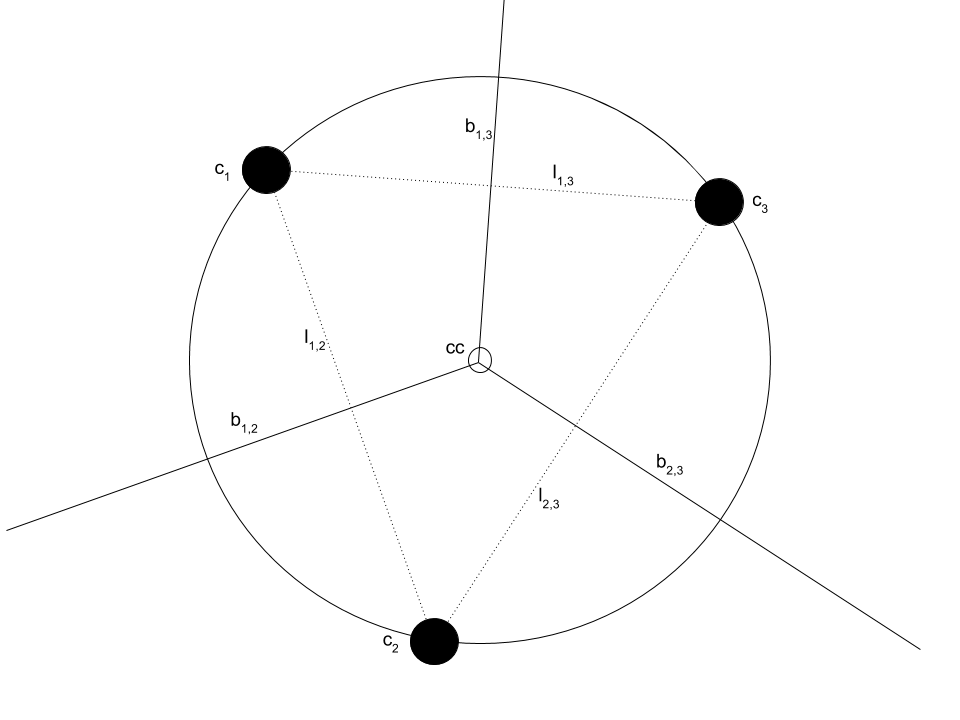
\includegraphics[width=0.8\textwidth]{Images/vor_triangle.png}
\caption{A Voronoi tessellation of three points ($c_1$, $c_2$ and $c_3$) with circumcentre ($cc$).}
\label{fig:vor_triangle}
\end{figure}
A list of the bisecting lines, the range of the points and the convex hull (which is yet to be determined) are returned.
\\
\\
For a range of two points, the bisecting line, $b_{1,2}$, is determined as the only line in the structure. The centres and $b_{1,2}$ are placed into one another's related centre list and the line is placed in a list as the only element. The line list, the range of the centres and their convex hull are returned.
\\
\\
The case of a single centre is excluded as the case of multiple centres divides the set of centres either into two equal subsets or two subsets differing in size by one. The second and third cases will catch sets of three or two centres and therefore the case of a single centre cannot be determined unless a set of a single is passed through initially. This is, however, meaningless as the Voronoi tessellation for this would be a single cell containing the entire space.

\subsection{Convex Hull}
The convex hull of a set of $n$ points, $P = {p_0,p_1,...,p_n}$, is defined as the smallest convex set that contains all the points of $P$. The convex set can be seen as a polygon where each vertex of the polygon is convex (has an internal angle less than $\pi$ radians). For the convex set to be minimal, the vertices of the convex set must lie on a subset of the points of $P$. A convex hull of $P$ can be determined in $O(n\log(n))$ time \citep{eddy1977new}. Figure \ref{fig:convexhull} shows an example of a convex hull.
\begin{figure}[H]
\centering
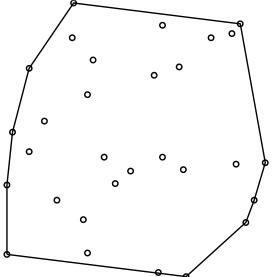
\includegraphics[width=0.5\textwidth]{Images/convexhull.png}
\caption[]{A convex hull of a set of points\footnotemark.}
\label{fig:convexhull}
\end{figure}
\footnotetext{Taken from \url{http://www.evanjones.ca/convexhulls.html}}
Andrew's monotone chain convex hull algorithm \citep{andrew1979another} was used to determine the convex hull of each subset of centres. The function is first passed a range of centres on which to operate. The centres must be ordered lexicographically, which was done before the Voronoi creation process was started. A list of zeros, twice the size of the number of centres in the range is created; this list holds the elements of the chain. The complete convex hull is calculated in two steps, with the first finding the upper hull and the second finding the lower hull.
\\
\\
The first centre, $c_0$, which is also the leftmost centre and the second centre in the range, $c_1$, are both added to the list. The rest of the range is iterated over, adding the next centre to our list, if the angle created by the three points at the end of the list $c_{j-1}$, $c_j$ and $c_{j+1}$, is less than $\pi$ radians. The three centres remain in the list and the next centre, $c_{j+2}$ is added. If the angle is greater than $\pi$ radians, the two centres at the end of the list, $c_j$ and $c_{j+1}$, are removed and the process continues by adding the next point, $c_{j+2}$. This continues until the rightmost centre, $c_n$, is reached, at which time the upper hull of the convex hull has been created.
\\
\\
To generate the lower hull, the same process is used, but the range is iterated over in reverse, starting at the rightmost centre, $c_n$, and ending at the leftmost, $c_0$.
\begin{figure}[H]
\centering
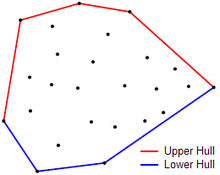
\includegraphics[width=0.5\textwidth]{Images/andrewmonotone.png}
\caption[]{A convex hull created using Andrew's monotone convex hull algorithm with the upper hull in red and the lower hull in blue\footnotemark.}
\label{fig:andrewmonotone}
\end{figure}
\footnotetext{Taken from \url{https://en.wikibooks.org/wiki/Algorithm_Implementation/Geometry/Convex_hull/Monotone_chain}}
Once the list has been populated with the centres of the lower and upper hulls, the monotone chain is formed. The chain is iterated over with each centre in the chain adding the preceding centre to its counter-clockwise parameter and the next point to its clockwise one.

\subsection{Voronoi Merge Function}
The merge begins by finding the upper and lower tangents, $t_u$ and $t_l$ respectively, of the sets $C_L$ and $C_R$. These tangent lines are defined as connections between the convex hulls of $C_L$ and $C_R$ such that they form part of the convex hull of the union of $C_L$ and $C_R$. Starting from the rightmost centre in $C_L$ and the leftmost centre in $C_R$, the algorithm finds the upper tangent by creating two sets of three centres, $(c^L_i,c^L_{i-1},c^R_j)$ and $(c^L_i,c^R_j,C^R_{j+1})$ where $c^L$ and $c^R$ indicate centres in $C_L$ and $C_R$, respectively. These overlapping sets must both satisfy the convex condition, i.e. the angle between these three centres must be less than $\pi$ radians. Once these conditions are met, $t_u$ is created between $C^L_i$ and $C^R_j$. The operation moves counter-clockwise on $C_L$ and clockwise on $C_R$. To find the lower tangent, $t_l$, the order is reversed with $C_L$ stepping clockwise and $C_R$ counter-clockwise. An example of this can be seen in Figure \ref{fig:v_merge1}.
\begin{figure}[H]
\centering
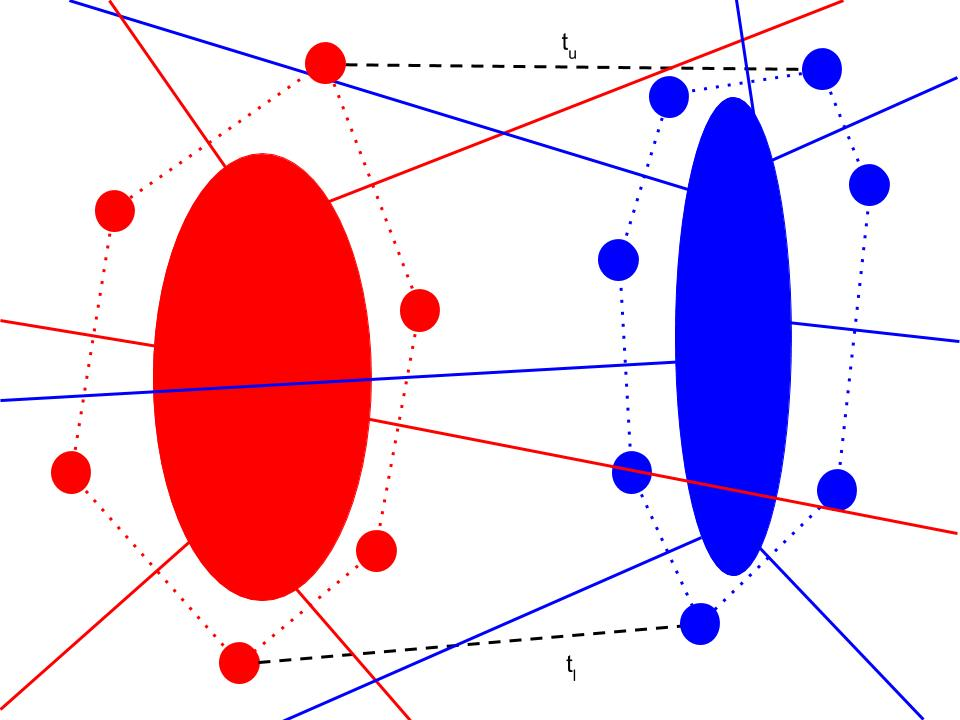
\includegraphics[width=0.6\textwidth]{Images/v_merge1.jpg}
\caption{Two neighbouring tessellations, $C_L$(red) and $C_R$(blue). Only centres affected by the merge on the convex hull and their bisecting lines are shown. The upper and lower tangents, $t_u$ and $t_l$ are shown in black.}
\label{fig:v_merge1}
\end{figure}
The upper tangent, $t_u$, is used to find the starting point of the polygonal chain used to merge the Voronoi. We start by creating an empty list, $HP$, which stores the line segments of the polygonal chain. The bisector of $t_u$, $b_0$, is used as the first line segment in the polygonal chain and is appended to HP. The endpoint of $t_u$ with the greatest $y$ value is determined, $c^u_0$, and a new tangent is generated with the lower centre, $c^u_1$, and a neighbour of $c^u_0$ in the same subset as $c^u_0$, not necessarily in the convex hull, so long as the related line to $c^u_0$ is both available and intercepts $b_0$. The bisecting line of $c^u_0$ and its chosen neighbour is appended to a list of lines which intercepts the polygonal chain, known as \textit{clip\_lines}. The bisector of $c^u_1$ and the chosen neighbour of $c^u_0$ is determined and appended to $HP$ and the process begins anew. An illustration of a step in the process can be seen in the transition from Figure \ref{fig:v_merge2} to Figure \ref{fig:v_merge3}.
\begin{figure}[H]
\centering
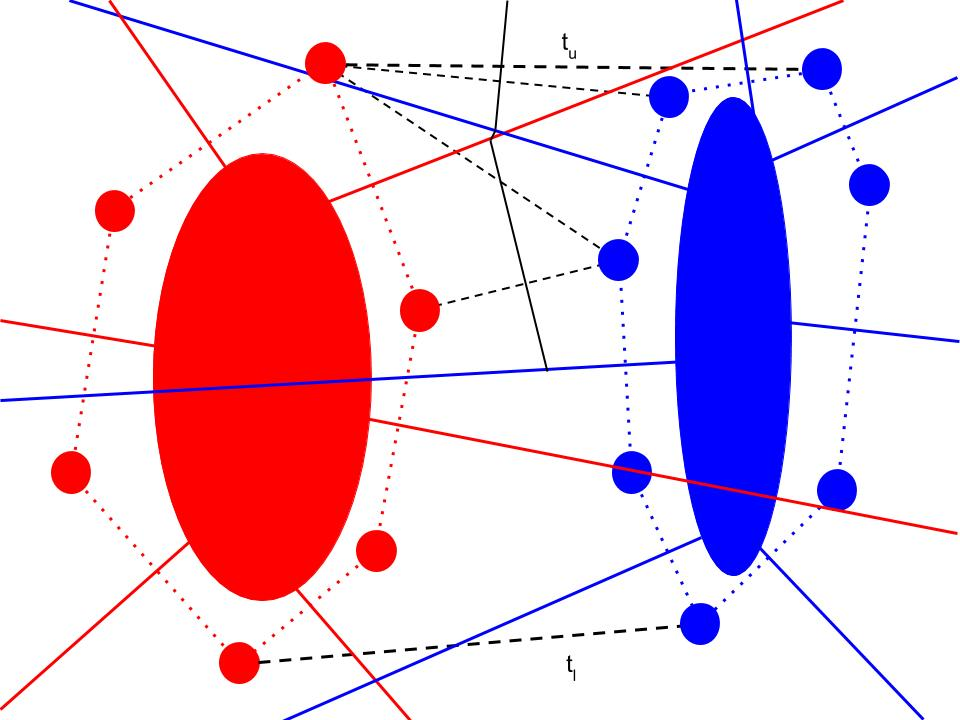
\includegraphics[width=0.6\textwidth]{Images/v_merge2.jpg}
\caption{Two neighbouring Voronoi tessellations merging: the dashed black lines depicting the tangent lines and the solid black line segments depict the growing polygonal chain.}
\label{fig:v_merge2}
\end{figure}
\begin{figure}[H]
\centering
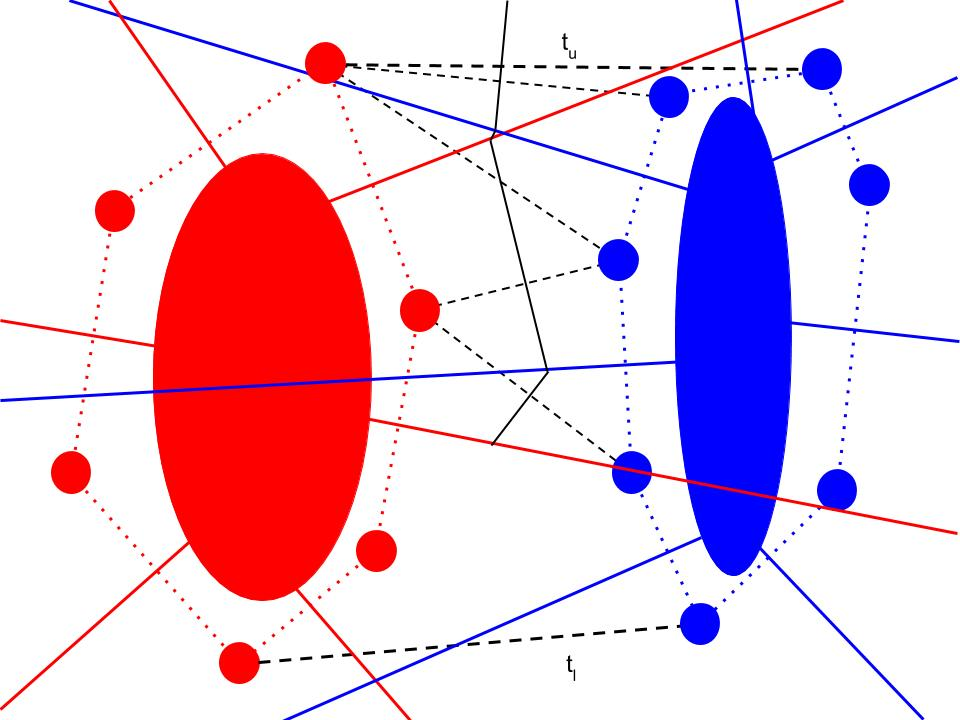
\includegraphics[width=0.6\textwidth]{Images/v_merge3.jpg}
\caption{Two neighbouring Voronoi tessellations continuing to merge.}
\label{fig:v_merge3}
\end{figure}
This process is repeated until the bisecting line of $t_l$ is determined,as shown in Figure \ref{fig:v_merge4}.
\begin{figure}[H]
\centering
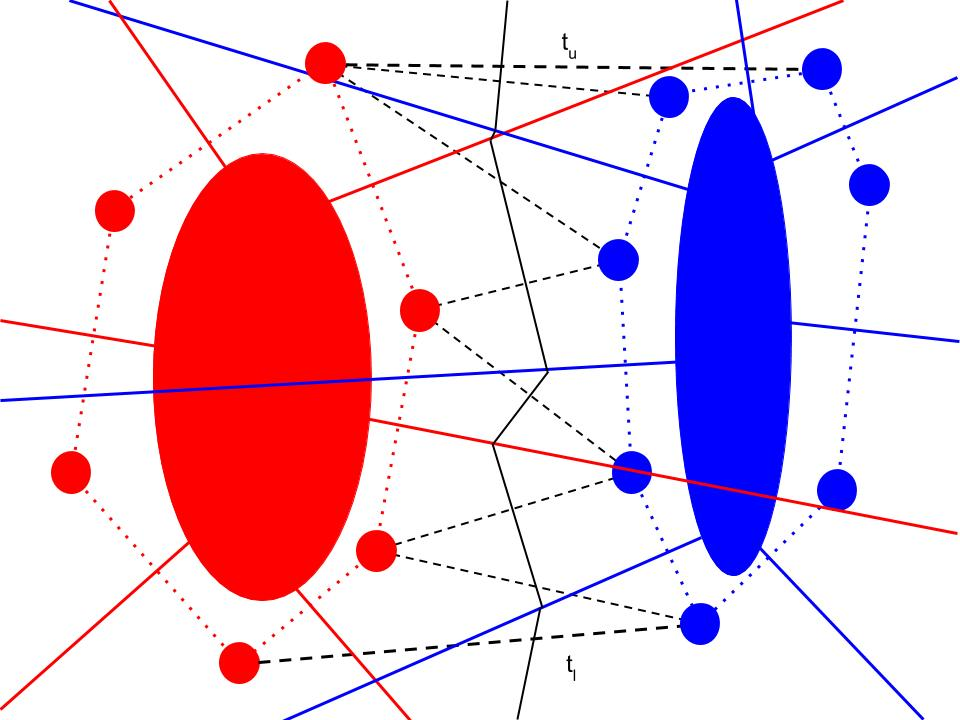
\includegraphics[width=0.6\textwidth]{Images/v_merge4.jpg}
\caption{A near complete Voronoi merge: the lower tangent $t_l$ has been reached by the polygonal chain depicted as solid black line segments.}
\label{fig:v_merge4}
\end{figure}
Once complete, we are left with a list, HP, which contains the bisecting lines between points in $C_L$ and $C_R$ and a list of bisecting lines from $C_L$ and $C_R$, \textit{clip\_lines}. The lines in $HP$ and the centres they bisect are added to the related lists of each of the centres they bisect. The lines in \textit{clip\_lines} are cut at their intercepts and all are appended to a list of lines to be passed back along with the range of points and the new convex hull of the combined Voronoi structure. A depiction of the two Voronoi tessellations with clipped lines can be seen in Figure \ref{fig:v_merge5}.
\begin{figure}[H]
\centering
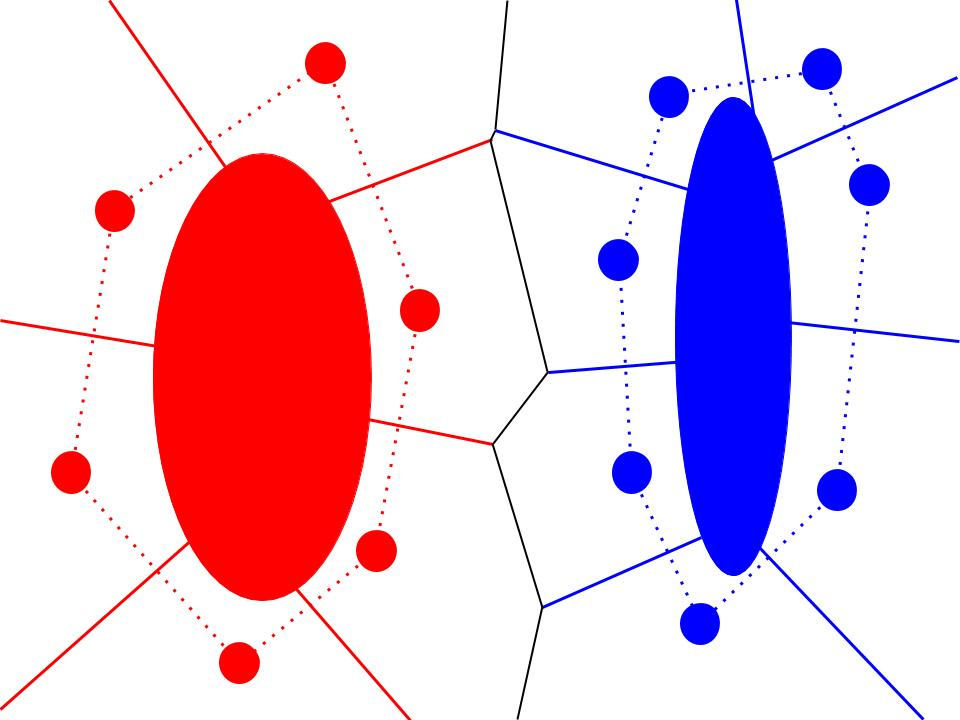
\includegraphics[width=0.6\textwidth]{Images/v_merge5.jpg}
\caption{A completed Voronoi merge, with clipped lines denoting the new cell dimensions.}
\label{fig:v_merge5}
\end{figure}
An example of a complete Voronoi Tessellation is illustrated in Figure \ref{fig:gen_voronoi}.
\begin{figure}[H]
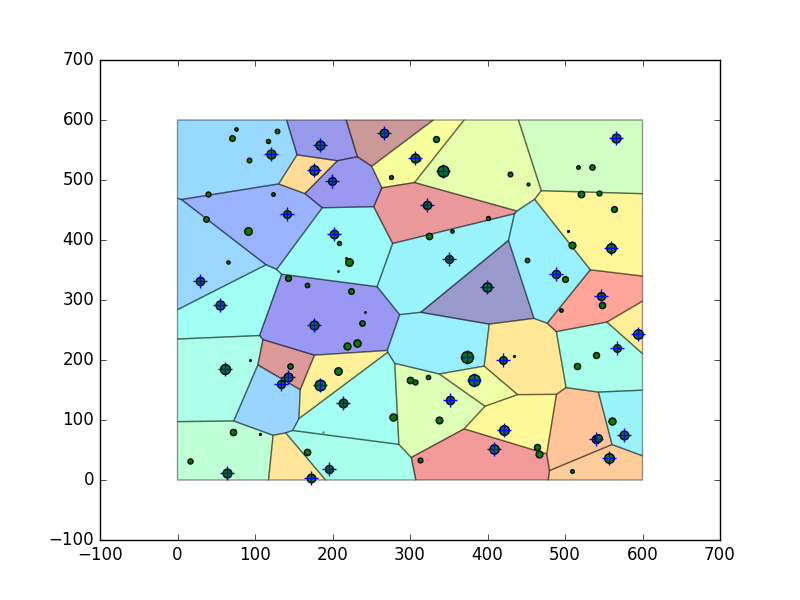
\includegraphics[width=\textwidth]{Images/recentre1.png}
\caption{A Voronoi tessellation generated by the divide and conquer algorithm with sources as circles and stars to represent the Voronoi centres.}
\label{fig:gen_voronoi}
\end{figure}
\subsection{Weighted Voronoi Tessellation}
An attempt was made to generate a weighted Voronoi tessellation using a distance transform which uses the intensities of the centres to redetermine the coordinates of the midpoint of the centres. This transform is defined in Equation (\ref{eq:w_dist}) where $z_1$ and $z_2$, and $\vec{x_1}$ and $\vec{x_2}$ are the intensities and coordinates of $c_1$ and $c_2$, respectively.
\begin{equation}\label{eq:w_dist}
	d'(c_1,c_2) = \frac{z_1}{z_1+z_2}\vec{x_1} + \frac{z_2}{z_1+z_2}\vec{x_2}
\end{equation}
This is an extension of the standard distance equation since, if $z_1=z_2$ we obtain
\begin{align*}
	d'(c_1,c_2) &= \frac{z_1}{z_1+z_2}\vec{x_1} + \frac{z_2}{z_1+z_2}\vec{x_2} \\
	d'(c_1,c_2) &= \frac{1}{2}\vec{x_1} + \frac{1}{2}\vec{x_2} \\ 
	d'(c_1,c_2) &= \frac{\vec{x_1} + \vec{x_2}}{2} \\
\end{align*}
Some complications were found in this method during the Voronoi merge process; weighted centres that are not close enough to the convex hull but due to their larger weighting still have cells that dominate areas of the hull were not included in the merging process and their line segments were not clipped or deactivated. Another problem is that this method generates undefined regions in the space, that is, regions where domains overlap due to conflicting weightings, an example of which can be seen in Figure \ref{fig:w_voronoi_issue}.
\begin{figure}[H]
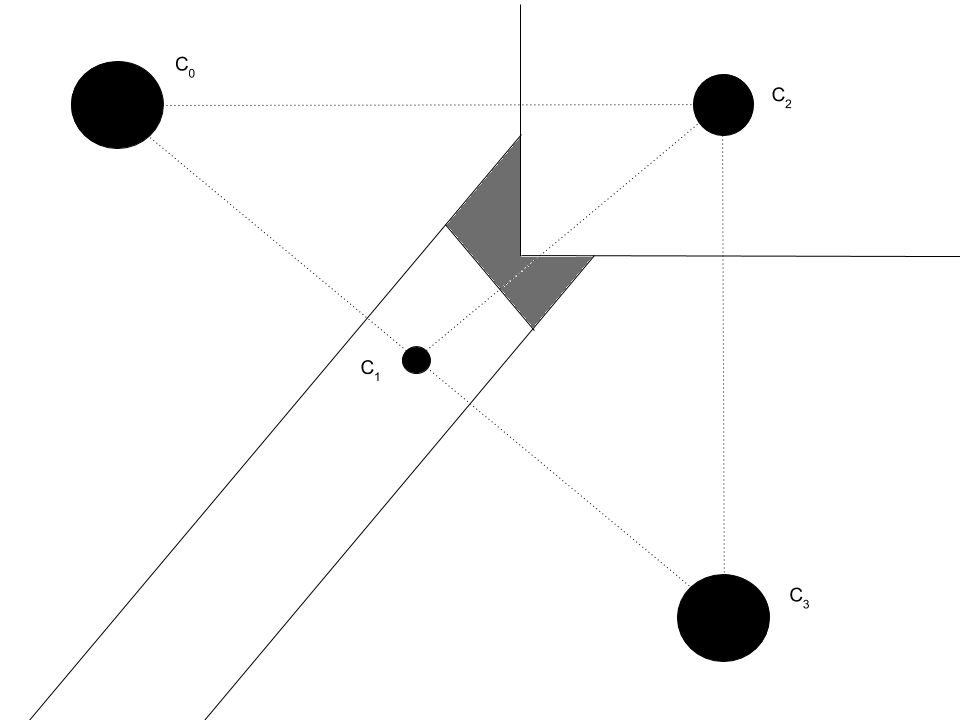
\includegraphics[width=0.5\textwidth]{Images/weighting_problem.png}
\centering
\caption{An unclassified area (grey) generated by a weighting conflict in $c_1$ and $c_2$.}
\label{fig:w_voronoi_issue}
\end{figure}
The figure shows a conflicting area between $c_1$ and $c_2$. It would be expected that $c_2$, with its higher intensity, would claim the area, but in doing so it would cross into the area that should be the domain of $c_0$ or $c_3$. It was for this reason that the choice to use the intensities to weight the Voronoi tessellation creation process was abandoned. Instead the intensities would be used to calculate the error and determine and generate cell merges. An example of a failed weighted Voronoi tessellation can be seen in Figure \ref{fig:w_voronoi}.
\begin{figure}[H]
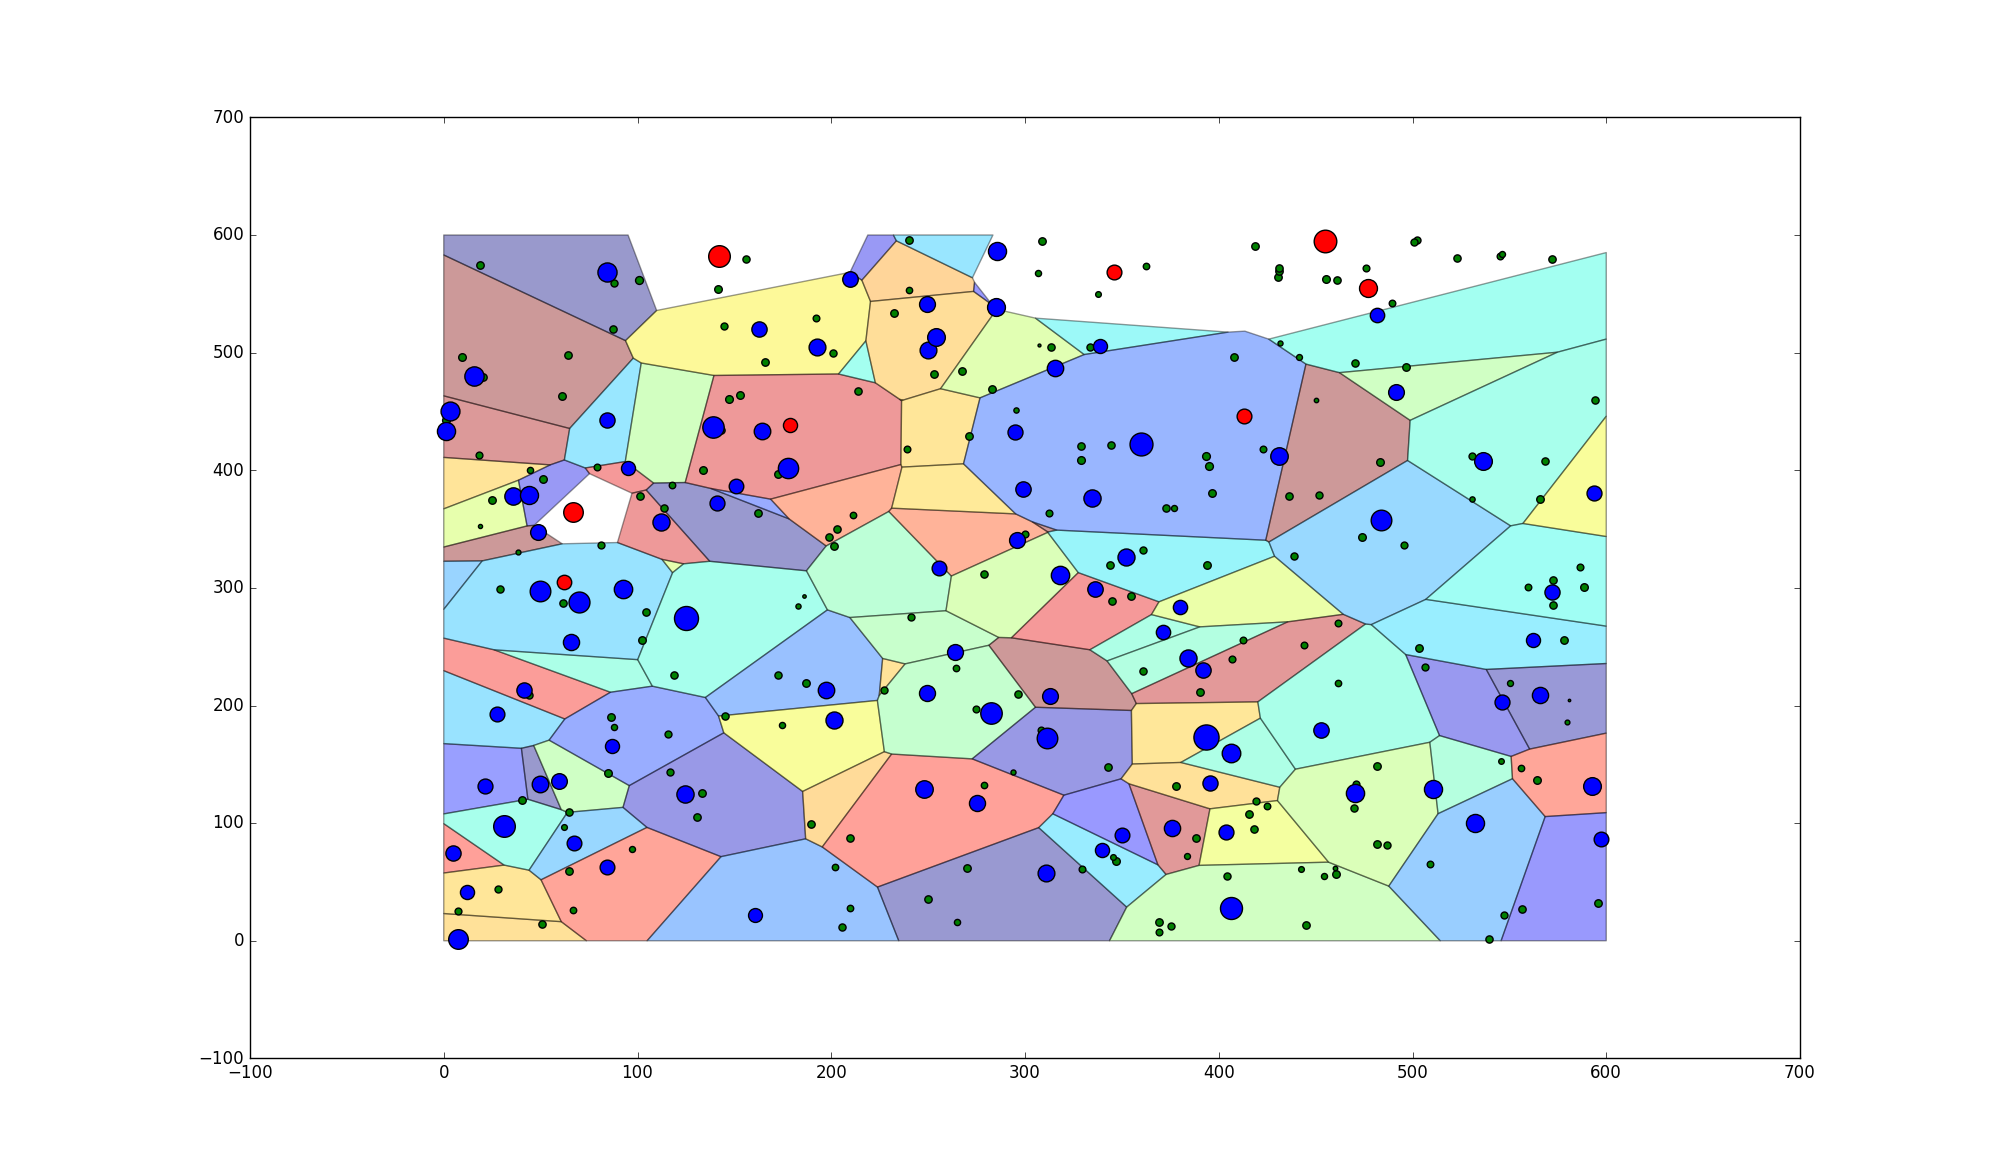
\includegraphics[width=\textwidth]{Images/weighted_voronoi.png}
\centering
\caption{A failed visualisation of a weighted Voronoi tessellation with centres in blue, sources in green and centres without cells in red.}
\label{fig:w_voronoi}
\end{figure}

\section{Cell Error}
Once the Voronoi tessellation has been determined, it is re-centred based on the weighted average of the points in the cell. Sources are added to cells by determining the cell centre which is closest to it using the standard distance equation:
\begin{equation}
d = \sqrt{(x_i - x_j)^2 + (y_i - y_j)^2},
\end{equation}
where $(x_i,y_i)$ is the location of a source in the plane and $(x_j,y_j)$ is the location of a centre. The closest centre is such that $d$ is minimum. For each source, $s_i$ we therefore seek its minimum distance, $d_i$, such that for a set of $n$ centres:
\begin{equation}
d_i = \min^n_j \sqrt{(x_i - x_j)^2 + (y_i - y_j)^2}.
\end{equation}
This is done to add the influence of weaker sources in the overall correction and is especially necessary when the cell is generated by a source slightly above the intensity threshold and contains a source slightly below the threshold. We seek a new weighted centre such that the error for a cell is minimum. The error for a cell containing $N$ sources is defined as
\begin{equation} \label{eq:cellerr}
	\epsilon_j = \sum^N_{i=1} z_i||\vec{x_i} - \vec{x_j}||^2,
\end{equation}
where $\vec{x_i} = (x_i,y_i)$ is the location, $z_i$ is the intensity of some source in the cell, and $\vec{x_j}$ is the location of the new centre. 
\\
\\
This error function has a local minimum at the point where its derivative with regard to $\vec{x_j}$ is zero, or
\begin{align*}
	\frac{d\epsilon}{d\vec{x_j}} &= \sum^N_{i=1} \frac{d}{d\vec{x_j}}z_i(||\vec{x_i}||^2 -2\vec{x_i}\cdot\vec{x_j} + ||\vec{x_j}||^2) \\
	&= \sum^N_{i=1} z_i(2\vec{x_i} - 2\vec{x_j}) = 0 \\
\end{align*}
or
\begin{equation*}
	2\sum^N_{i=1} z_i\vec{x_i} = 2\sum^N_{i=1}z_i\vec{x_j}.
\end{equation*}
Since $\vec{x_j}$ is not dependent on the sum, it can be removed and the equation reordered to give
\begin{equation}
	\vec{x_j} = \frac{\sum^N_{i=1} z_i\vec{x_i}}{\sum^N_{i=1}z_i}.
\end{equation}
From this, the new centre is determined. The intensity of the centre is determined as the sum of the intensities in the cell, or:
\begin{equation}
	z_j = \sum^N_{i=1} z_i.
\end{equation}
Once the cell's new centre has been obtained, its error is calculated using Equation (\ref{eq:cellerr}). An example of centre correction can be seen in the transition from Figure \ref{fig:recen1} to Figure \ref{fig:recen2}.
\begin{figure}[H]
  \centering
  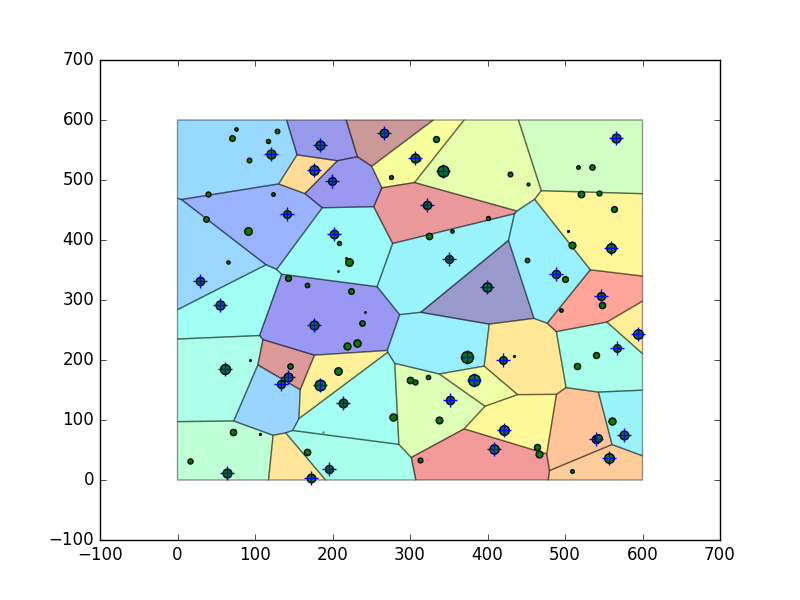
\includegraphics[width=0.8\textwidth]{Images/recentre1.png}
  \caption{Tessellation with high intensity sources as centres.}
  \label{fig:recen1}
\end{figure}
\begin{figure}[H]
  \centering
  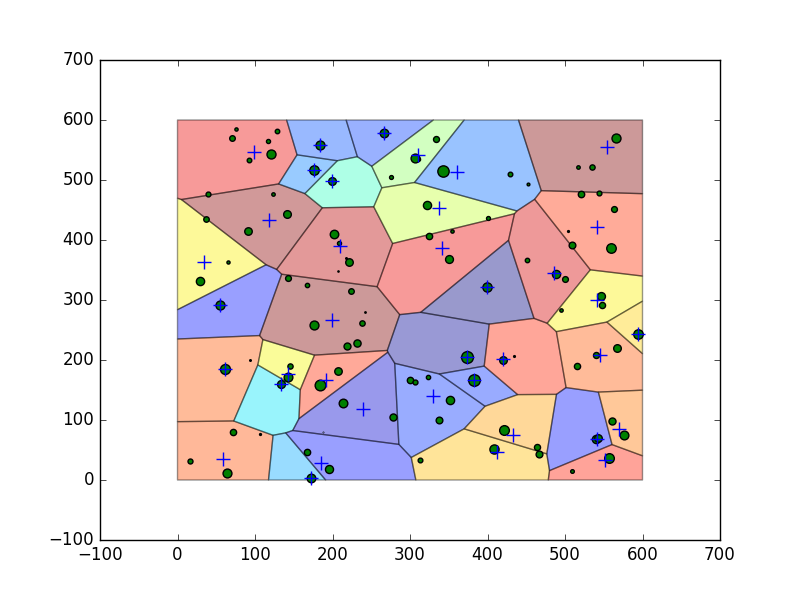
\includegraphics[width=0.8\textwidth]{Images/recentre2.png}
  \caption{Tessellation with the weighted average of the sources in the cells as their centres.}
  \label{fig:recen2}
\end{figure}
\section{Cell Merge}\label{des:sec:merge}
The cell merge process is iterative and is dependent on the total sum of the error of the cells, $E$. Initially, this error is relatively low as multiple cells are generated with one or very few sources contained in each cell. To keep the maximum error threshold relative, unless it is given as an input by the user, it is calculated as the product of the set standard deviation ($\sigma$), the size of the plane ($x_{plane},y_{plane}$) and the number of sources in the plane ($|S|$) or 
\begin{equation}\label{des:eq:maxerr}
 E_{max} = \sigma x_{plane}y_{plane}|S|.
\end{equation}
The process begins by summing the errors of the cells and iterates through the process of finding the best merge, checking if implementing the best merge exceeds the maximum error threshold and, if not, implementing the best merge.

\subsection{Obtaining the Best Merge}
The best merge is obtained by iterating over the list of centres and, for each centre, testing it with its active neighbouring centres.
\\
\\
The merge test works by calculating a new centre, $c_{new} = (\vec{X},Z)$, determined by two existing centres, $c_1$ and $c_2$, with intensities $z_1$ and $z_2$, and positions $\vec{x_1}$ and $\vec{x_2}$, respectively, as
\begin{equation} \label{eq:merge_centre}
	\vec{X} = t\vec{x_1} + (1-t)\vec{x_2} \text{  with  } t = \frac{z_1}{z_1 + z_2}.
\end{equation}
The new weight for the merged centre is defined as
\begin{equation}
	Z = z_1 + z_2.
\end{equation}
Since $x_1$ and $x_2$ are centred sums of the positions of the sources in their cells, expanding them to their original forms yields
\begin{equation*}
\vec{x_1} = \frac{\sum^N_{i=1} z_{1i}\vec{x_{1i}}}{\sum^N_{i=1}z_{1i}} \text{  and  } \vec{z_2} = \frac{\sum^M_{i=1} z_{2i}\vec{x_{2i}}}{\sum^M_{i=1}z_{2i}}.
\end{equation*}
Note that:
\begin{equation*}
	z_j = \sum^N_{i=1}z_{ji}.
\end{equation*}
Substituting these into Equation (\ref{eq:merge_centre}), we obtain
\begin{align*}
	\vec{X}	&= t\vec{x_1} + (1-t)\vec{x_2} \\
		&= \frac{z_1}{z_1 + z_2}\frac{\sum^N_{i=1} z_{1i}\vec{x_{1i}}}{z_1} + (\frac{z_1 + z_2}{z_1 + z_2} - \frac{z_1}{z_1 + z_2})\frac{\sum^M_{i=1} z_{2i}\vec{x_{2i}}}{z_2} \\
		&= \frac{\sum^N_{i=1} z_{1i}\vec{x_{1i}}}{z_1 + z_2} + \frac{\sum^M_{i=1} z_{2i}\vec{x_{2i}}}{z_1 + z_2} \\
		&= \frac{\sum^N_{i=1} z_{1i}\vec{x_{1i}} + \sum^M_{i=1} z_{2i}\vec{x_{2i}}}{z_1 + z_2} \\
		&= \frac{\sum^N_{i=1} z_{1i}\vec{x_{1i}} + \sum^M_{i=1} z_{2i}\vec{x_{2i}}}{\sum^N_{i=1}z_{1i} + \sum^M_{i=1}z_{2i}}.
\end{align*}
This shows that Equation (\ref{eq:merge_centre}) is equivalent to finding the centre of all the sources in both $x_1$ and $x_2$.
\\
\\
Once the new centre has been found, the error must be determined by summing the square of the weighted distances to the new centre from each source. Once determined, the new centres coordinates and intensity, as well as the new error are returned. The error itself is not compared to find the best merge, but rather the change in error, that is, the merge that produces the lowest increase in the error. This is done by taking the tested merge error and subtracting from it the errors of the centres used to generate it; i.e., we seek $\Delta_{i,j}$ such that for some cells $c_i$ and $c_2j$, the comparison with the error of the merged cell, $c_{i,j}$ is:
\begin{equation}\label{des:eq:delta}
	\Delta_{i,j} = \min^n_{i = 1}\min^n_{j = 1, i \neq j}c_{i,j} - (c_i + c_j).
\end{equation}
Once found, the result is stored along with the new coordinates of the centre, $c_{i,j}$ and the centres used to generate it.
\\
\\
Once the best merge has been found, it must be determined whether the new sum of errors exceeds the threshold, i.e. $E + \Delta_{i,j} \geq E_{max}$. If it does, the merge process is halted and the Voronoi structure is returned. If the threshold is set too high, it may occur that all the cells merge into a single cell. In this case, the process is again halted as no best merge could be found as the threshold was set too high for the system. The Voronoi structure is returned as only the set of sources and a single centre with no bisecting lines remaining and so no merged Voronoi can be generated. If the system finds a valid merge which is still less than the threshold, it adds the difference in the merge error to the total error and executes the merge.

\subsection{Executing the Merge}
The merge execution algorithm takes in the new coordinates and intensity, $\vec{X}$, the new error, $Z$, as well as the centre, $c_1$, and the related centre with which it is to be merged, $c_2$. The algorithm starts by setting the coordinates and intensity of $c_1$ to those of $c_{1,2} = (\vec{X},Z)$. It deprecates the line relating $c_1$ to $c_2$ and appends the list of sources in $c_2$ to that of $c_1$. The error of $c_1$, $z_1$, is set to that of the new error, $Z$. Centre $c_2$ and its list of consumed centres are added to the list of consumed centres of $c_1$. Finally, the list of centres is iterated over and any centre which references $c_2$ is changed to reference $c_1$ and all lines which relate other centres to $c_2$ are changed to relate to $c_1$ instead. Once this is complete, the process of finding the best merge restarts until the error threshold is reached.
\\
\\
The transition from Figure \ref{fig:1merge1} to Figure \ref{fig:1merge2} shows the effects of a single merge. The weighted distance between the merged centres in Figure \ref{fig:1merge1} is less than those of all other neighbouring centre pairs.
\begin{figure}[H]
  \centering
  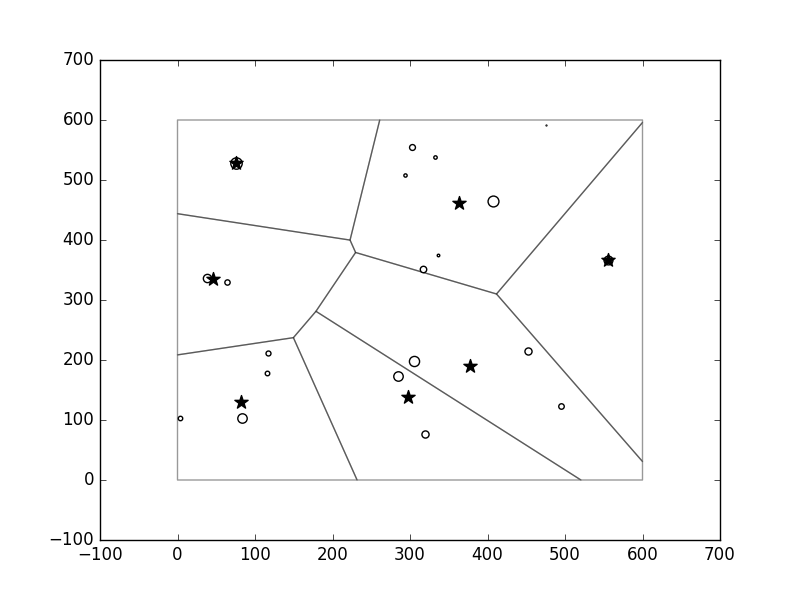
\includegraphics[width=0.8\textwidth]{Images/1merge1.png}
  \caption{Re-centred Voronoi before merge.}
  \label{fig:1merge1}
\end{figure}
\begin{figure}[H]
\centering
  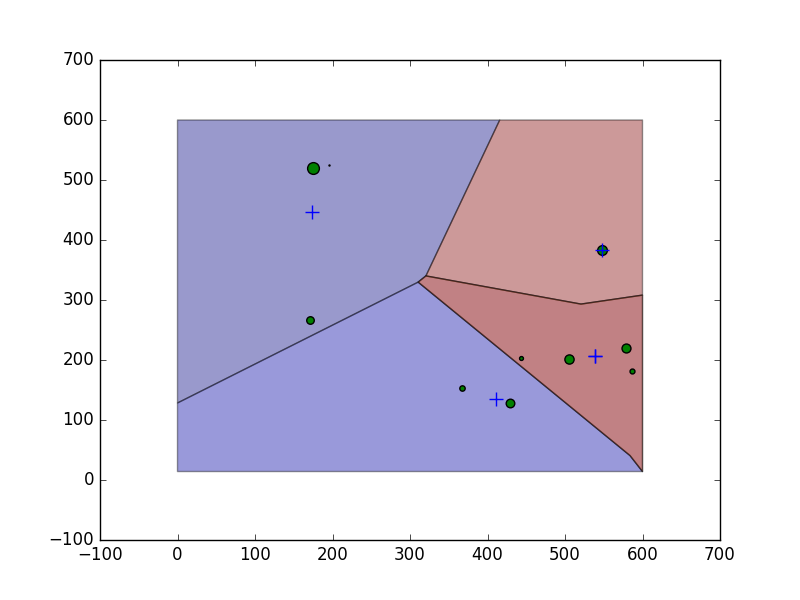
\includegraphics[width=0.8\textwidth]{Images/1merge2.png}
  \caption{Re-centred Voronoi after single merge.}
  \label{fig:1merge2}
\end{figure}
\begin{figure}[H]
\centering
  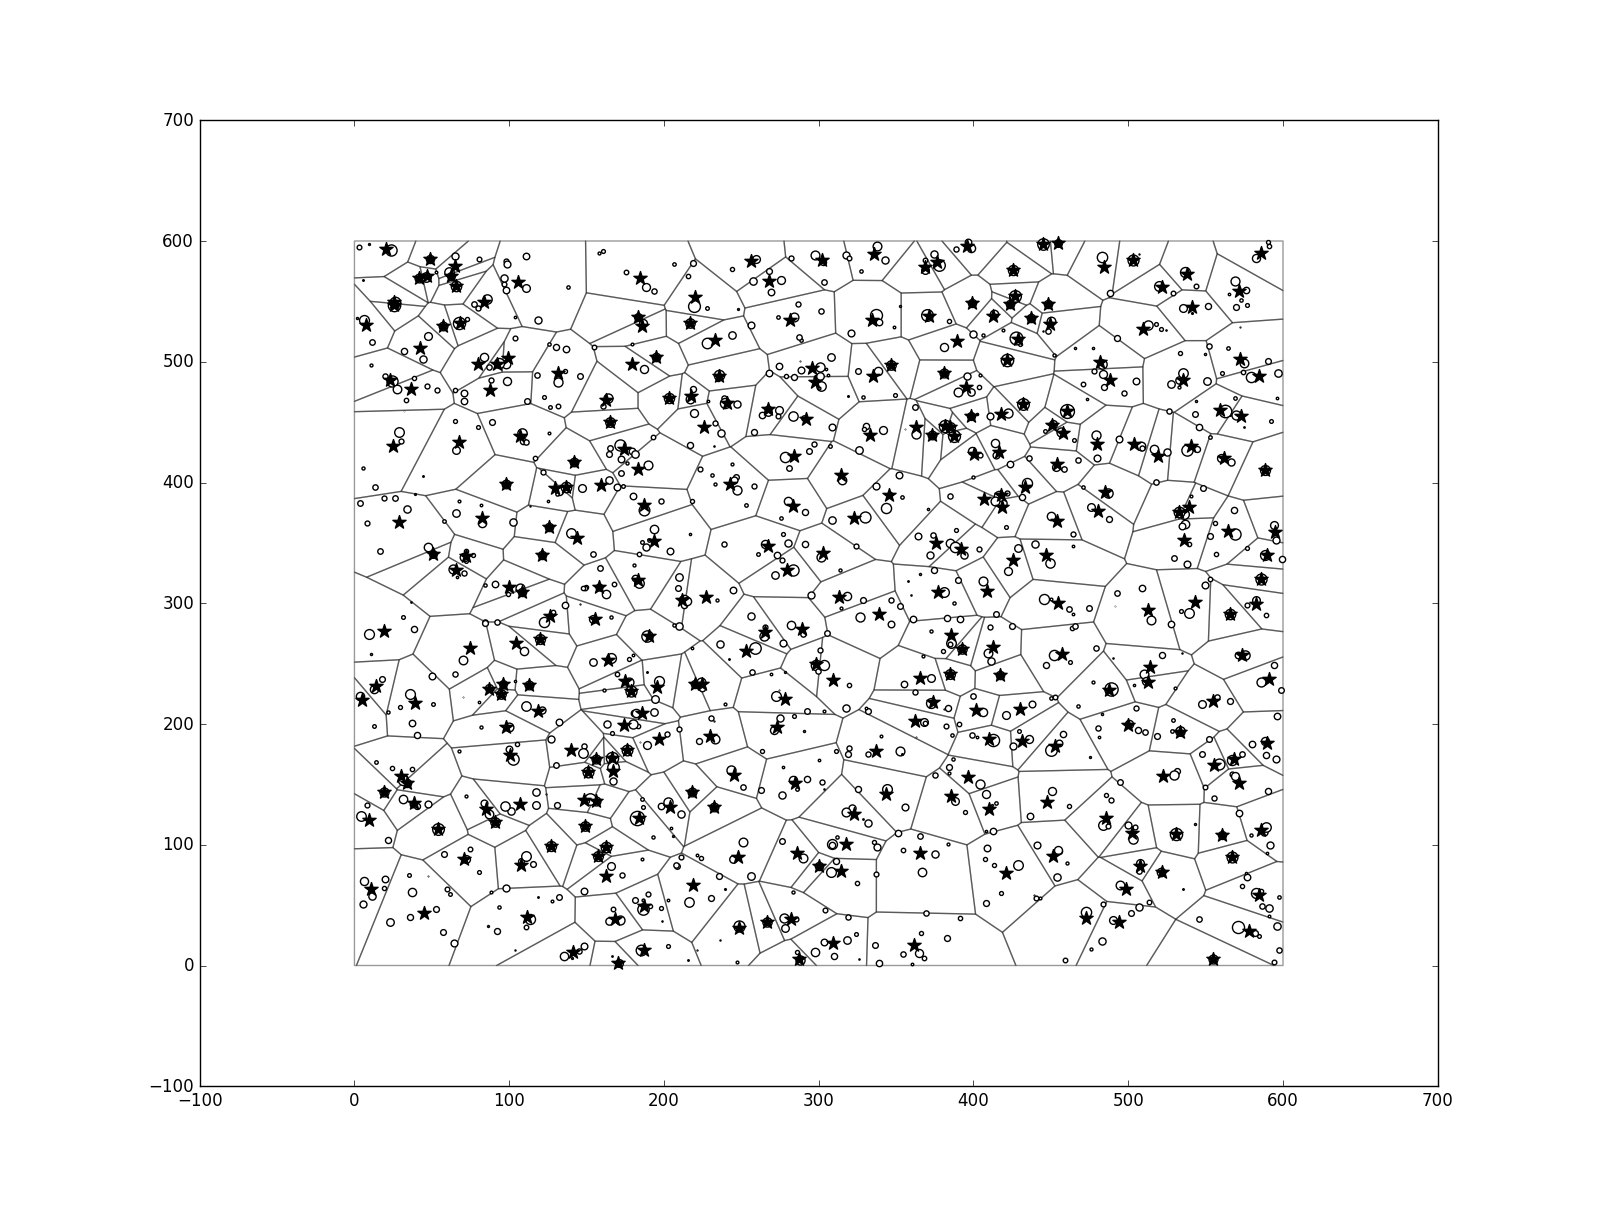
\includegraphics[width=0.8\linewidth]{Images/merge1.png}
  \caption{Re-centred Voronoi with 1000 sources and 301 centres before merge.}
  \label{fig:merge1}
\end{figure}
\begin{figure}[H]
\centering
  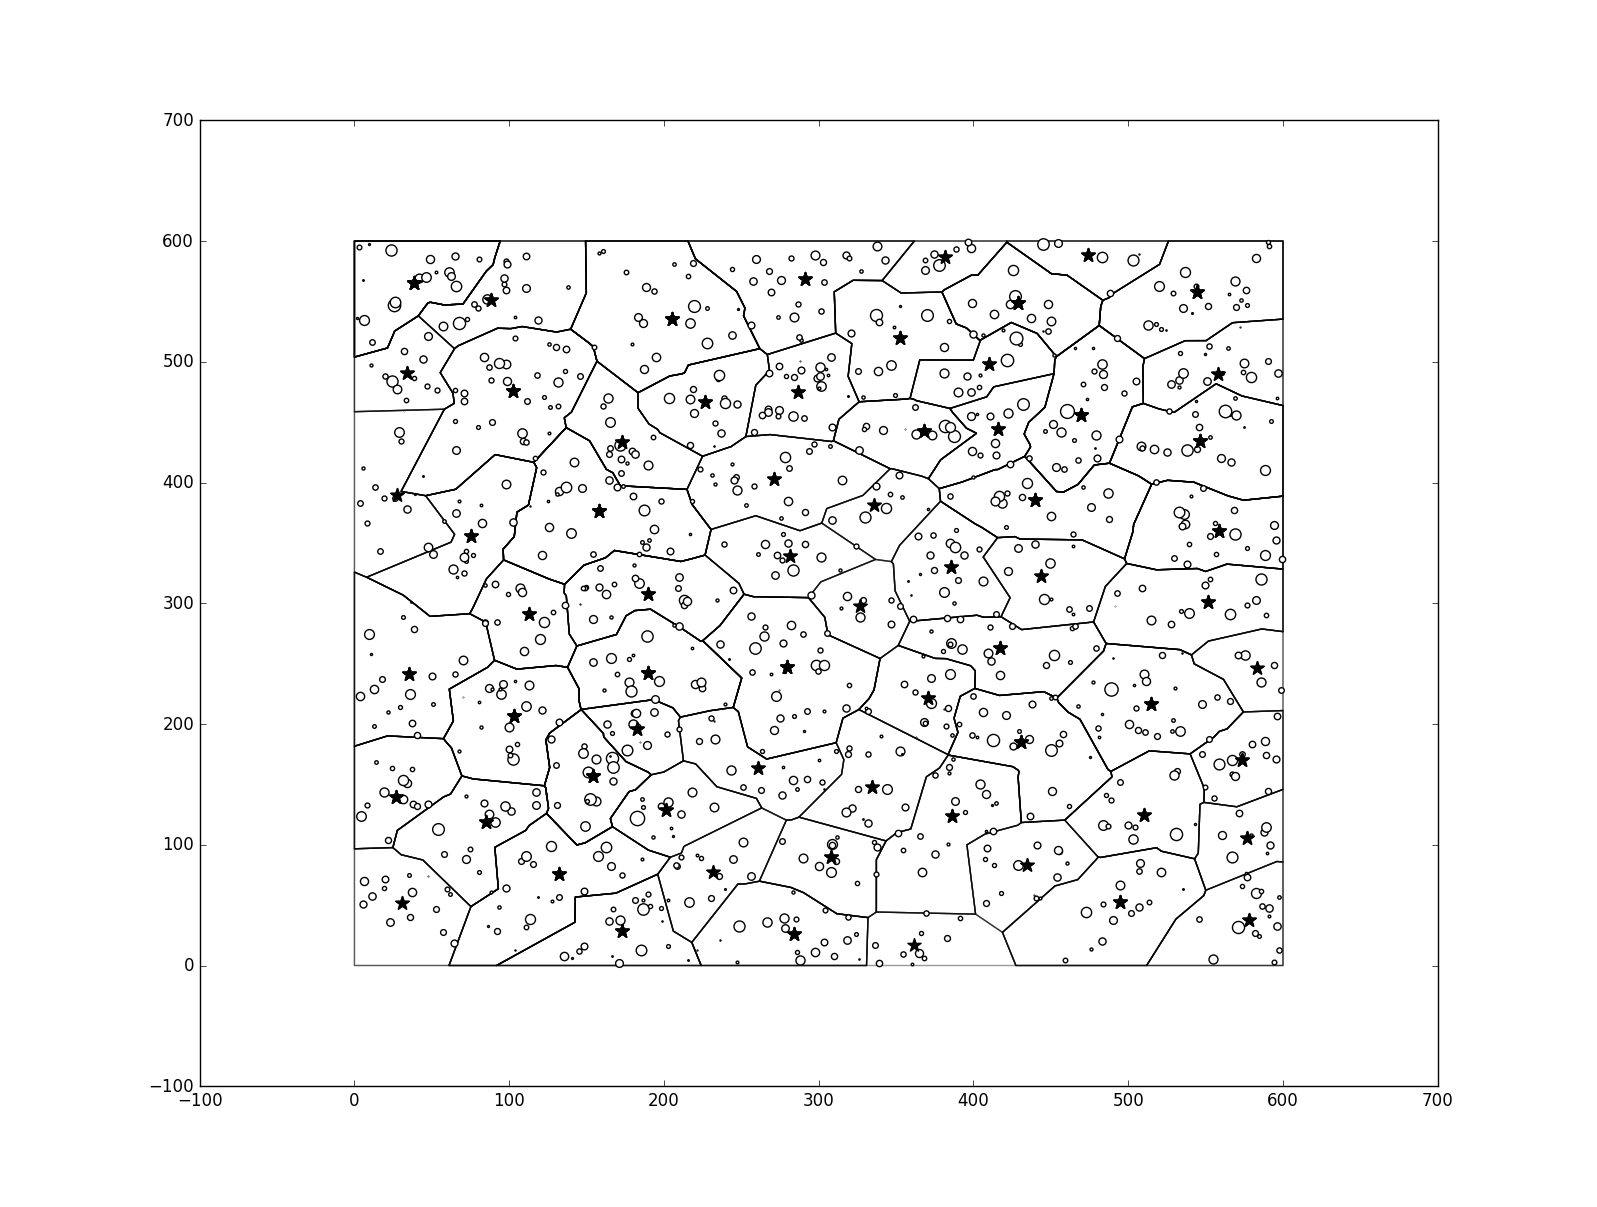
\includegraphics[width=0.8\linewidth]{Images/merge2.png}
  \caption{Re-centred Voronoi with 1000 sources and 64 centres after completing the merge process.}
  \label{fig:merge2}
\end{figure}
Figure \ref{fig:merge1} shows an initial Voronoi tessellation while Figure \ref{fig:merge2} shows its merged structure once the error threshold has been reached. The latter figure has larger structures with cells generally being more convex depending on the layout of sources in the cell.

\bibliography{Thesis_bib}
\bibliographystyle{ruauthordate}

\end{document}